\documentclass[../DefinizioneDiProdotto.tex]{subfiles}

\begin{document}

\section{Diagrammi di sequenza}
	In questa sezione vengono descritte e rappresentate tramite diagrammi di sequenza UML le sequenze di azioni ritenute più significative con lo scopo di facilitare la comprensione delle comunicazioni tra oggetti facenti parte dell'applicativo. Per quest'ultimo motivo i diagrammi di sequenza non rappresentano l'effettiva realtà ma una versione semplificata e che non rifletterà in tutto e per tutto l'implementazione finale.

	\subsection{Sessione ospite}
	Nella seguente tabella viene riportata la sequenza generale dell'interazione con il sistema dove l'attivazione viene eseguita mediante il Component StartStop. Il contenuto è riferito alla tipologia della domanda e non al cotenuto di essa. La sequenza descritta in alcuni punti potrà variare in numero o nell'ordine. Dall'interazione 0 (attivazione) all'interazione 3 (richiesta interlocutore) l'ordine non potrà essere modificato dall'amministratore, questo per riconoscere l'ospite anche in caso di modifiche alle domande poste. Inoltre la disattivazione sarà sempre l'operazione finale.

	\begin{longtable} [c] {
 >{\centering}p{1.5cm}
 p{2cm}
 p{6cm}
 p{5cm} }
 \toprule
 \textbf{Ordine} & \textbf{Descrizione azione} & \textbf{Descrizione interazione assistente virtuale} & \textbf{Descrizione interazione ospite} \\
 \midrule
 \arrayrulecolor{gray}
 0 & Attivazione & L'ospite attiva l'assistente virtuale tramite comando vocale invocando la keyword di Alexa specificata nella Skill \\
 \addlinespace[0.4em]
 \midrule
 \addlinespace[0.4em]
 1 & Richiesta azienda & L'assistente virtuale chiede all'ospite l'azienda di appartenenza & L'ospite pronuncia un nome \\
 \addlinespace[0.4em]
 \midrule
 \addlinespace[0.4em]
 2 & Richiesta proprio nominativo & L'assistente virtuale chiede all'ospite il proprio nome e cognome & L'ospite pronuncia un nominativo (nome e cognome) \\
 \addlinespace[0.4em]
 \midrule
 \addlinespace[0.4em]
 3 & Richiesta interlocutore & L'assistente virtuale chiede all'ospite chi desidera incontrare & L'ospite pronuncia un nominativo \\
 \addlinespace[0.4em]
 \midrule
 \addlinespace[0.4em]
 4 & Richiesta materiale & L'assistente virtuale chiede all'ospite se necessita di eventuale materiale per l'incontro & L'ospite pronuncia la parola "yes", seguito da una frase \\
 \addlinespace[0.4em]
 \midrule
 \addlinespace[0.4em]
 5 & Richiesta caffè & L'assistente virtuale chiede all'ospite se desidera un caffè durante l'attesa & L'ospite pronuncia la parola "yes" \\
 \addlinespace[0.4em]
 \midrule
 \addlinespace[0.4em]
 6 & Richiesta intrattenimento & L'assistente virtuale intrattiene l'ospite con alcuni argomenti, quali il meteo, le news e alcune barzellette & L'ospite pronuncia una parola tra "weather", "news", "jokes", seguito da una frase \\
 \addlinespace[0.4em]
 \midrule
 \addlinespace[0.4em]
 6.1 & Richiesta luogo & L'assistente virtuale chiede all'ospite di quale luogo desidera sapere il meteo & L'ospite pronuncia una parola \\
 \addlinespace[0.4em]
 \midrule
 \addlinespace[0.4em]
 6.2 & Richiesta genere & L'assistente virtuale chiede all'ospite il genere di notizie delle quali vuole essere informato & L'ospite pronuncia una parola \\
 \addlinespace[0.4em]
 \midrule
 \addlinespace[0.4em]
 7 & Disattivazione & Disattivazione & L'ospite pronuncia "Grazie Alexa, è tutto" \\
 \arrayrulecolor{black}
 \addlinespace[0.5em]
 \bottomrule
 \caption{Workflow interazione ospite}
\end{longtable}

	
	\subsection{\texttt{Alto livello Administration}}
	\begin{figure}[!h]
		\centering
		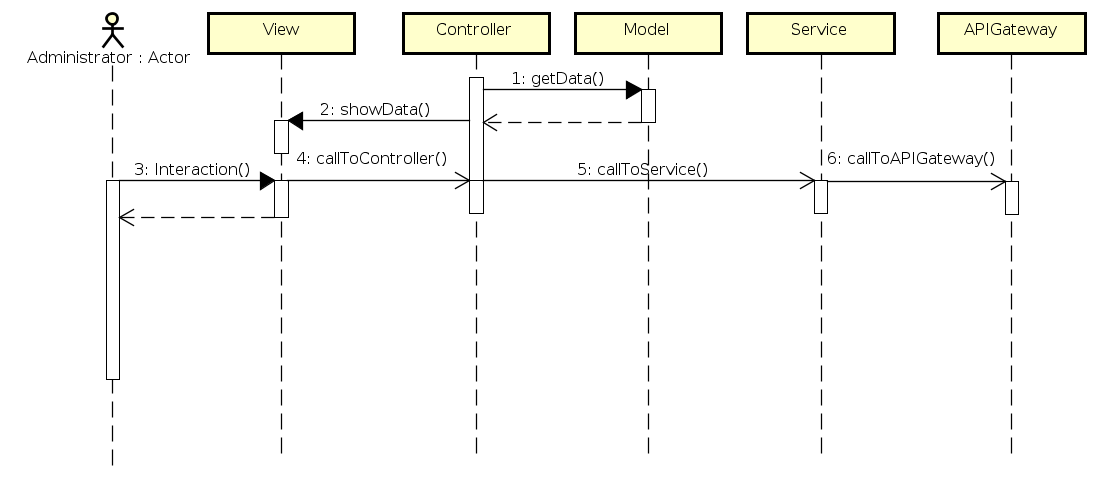
\includegraphics[width=\textwidth]{DiagrammiSequenza/DiagrammaSequenzaGeneraleAdmin.png}
		\caption{Diagramma di sequenza - \texttt{Alto livello Administration }}
	\end{figure}
	\begin{description}
		\item [Descrizione] Nel diagramma di sequenza sopra riportato  vengono illustrate le interazioni principali tra l'amministratore ed il sistema.
	\end{description}

	\subsection{\texttt{Front-End}}
		\subsubsection{\texttt{Front-End :: AdministrationView :: AdminComponents :: Login}}
		\begin{figure}[!h]
			\centering
			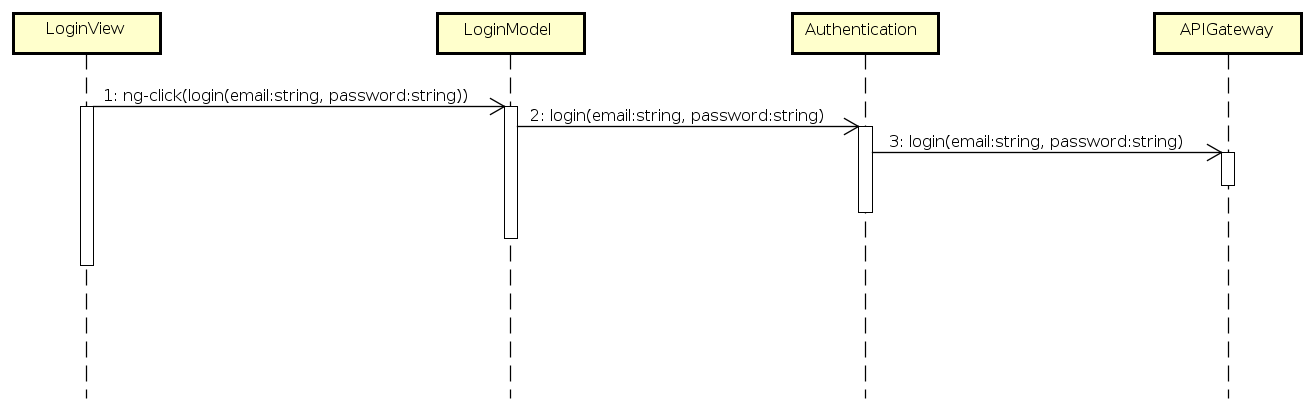
\includegraphics[width=\textwidth]{DiagrammiSequenza/Front-End/AdministrationView/Login.png}
			\caption{Diagramma di sequenza - \texttt{Front-End :: AdministrationView :: AdminComponents :: Login} }
		\end{figure}
		\begin{description}
			\item [Descrizione] Il diagramma di sequenza sopra riportato illustra l'operazione di login da parte dell'amministratore. Tramite il comando di Angular2 ng-click, viene effettua una chiamata API per autenticare l'amministratore nel sistema.
			\item [Permessi] Amministratore non autenticato.
	\end{description}

		\newpage
		\subsubsection{\texttt{Front-End :: AdministrationView :: AdminComponents :: Logout}}
		\begin{figure}[!h]
			\centering
			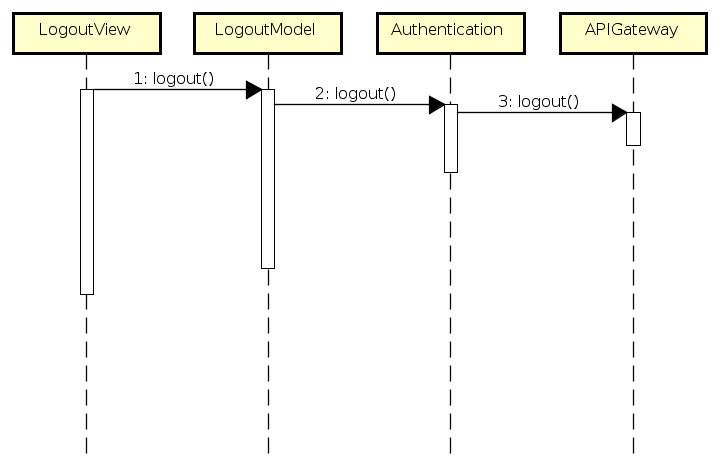
\includegraphics[width=\textwidth]{DiagrammiSequenza/Front-End/AdministrationView/Logout.png}
			\caption{Diagramma di sequenza - \texttt{Front-End :: AdministrationView :: AdminComponents :: Logout }}
		\end{figure}
		\begin{description}
			\item [Descrizione] Il diagramma di sequenza sopra riportato illustra l'operazione di logout da parte dell'amministratore. Tramite il comando di Angular2 ng-click, viene effettua una chiamata API per terminare la sessione dell'amministratore dal sistema.
			\item [Permessi] Amministratore autenticato.
		\end{description}

		\subsubsection{\texttt{Front-End :: AdministrationView :: AdminComponents :: RecoveryPassword}}
		\begin{figure}[!h]
			\centering
			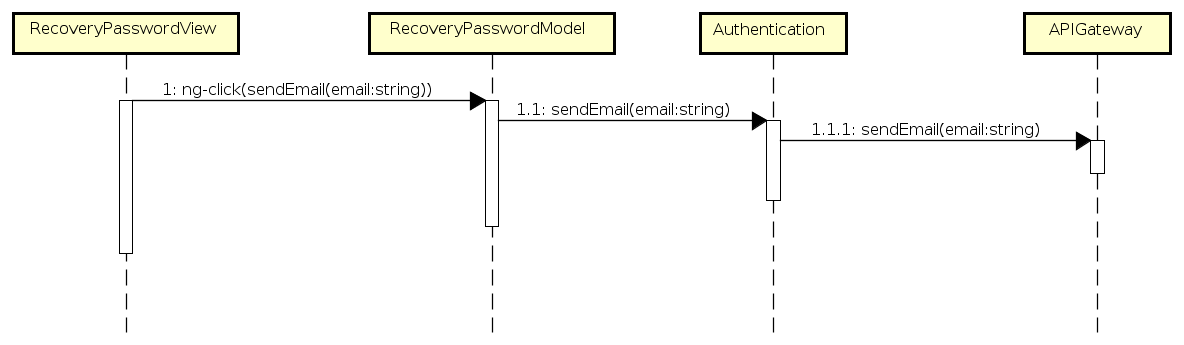
\includegraphics[width=\textwidth]{DiagrammiSequenza/Front-End/AdministrationView/RecoveryPassword.png}
			\caption{Diagramma di sequenza - \texttt{Front-End :: AdministrationView :: AdminComponents :: RecoveryPassword}}
		\end{figure}
		\begin{description}
			\item [Descrizione] Il diagramma di sequenza illustra l'operazione di recupero della password da parte dell'amministratore.
			\item [Permessi] Amministratore non autenticato.
		\end{description}

		\subsubsection{\texttt{Front-End :: AdministrationView :: AdminComponents :: ManageProfile}}
		\begin{figure}[!h]
			\centering
			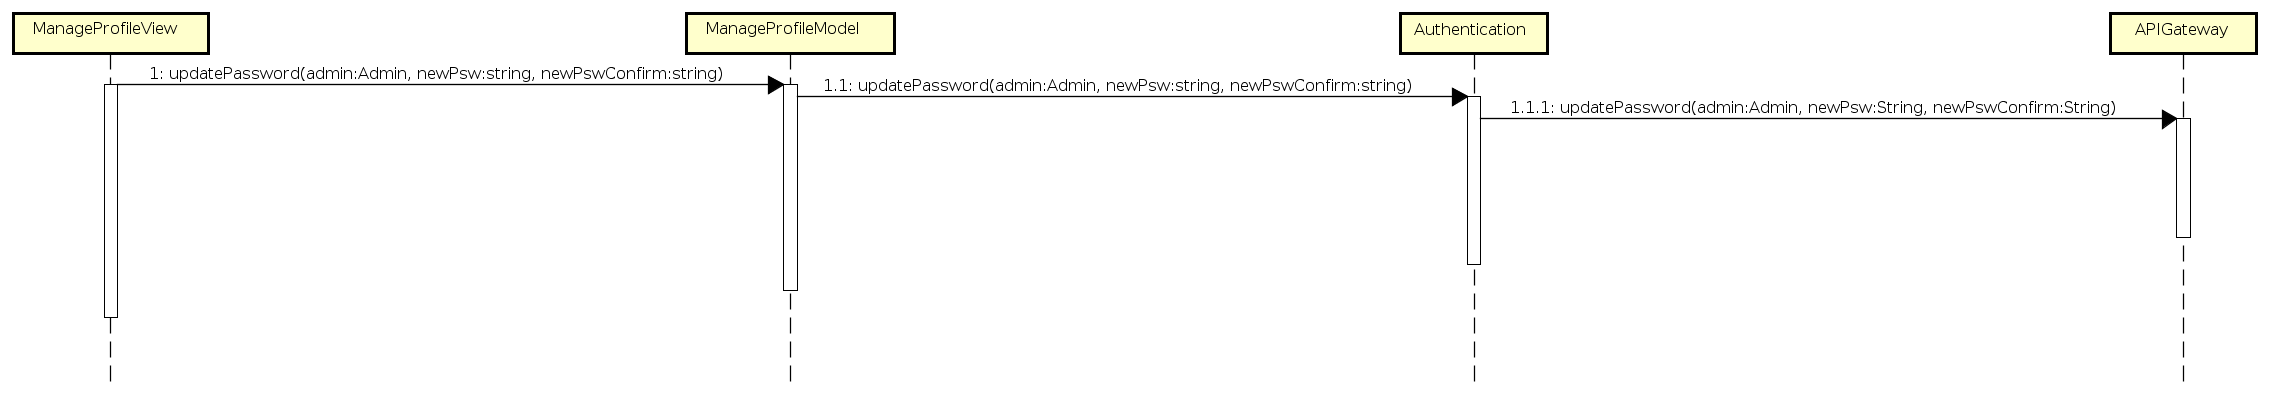
\includegraphics[width=\textwidth]{DiagrammiSequenza/Front-End/AdministrationView/ManageProfile.png}
			\caption{Diagramma di sequenza - \texttt{Front-End :: AdministrationView :: AdminComponents :: ManageProfile }}
		\end{figure}
		\begin{description}
			\item [Descrizione] Il diagramma di sequenza sopra riportato illustra l'operazione di gestione del proprio profilo da parte dell'amministratore.
			\item [Permessi] Amministratore autenticato.
		\end{description}

		\subsubsection{\texttt{Front-End :: AdministrationView :: AdminComponents :: ManageAdministrators}}
		\begin{figure}[!h]
			\centering
			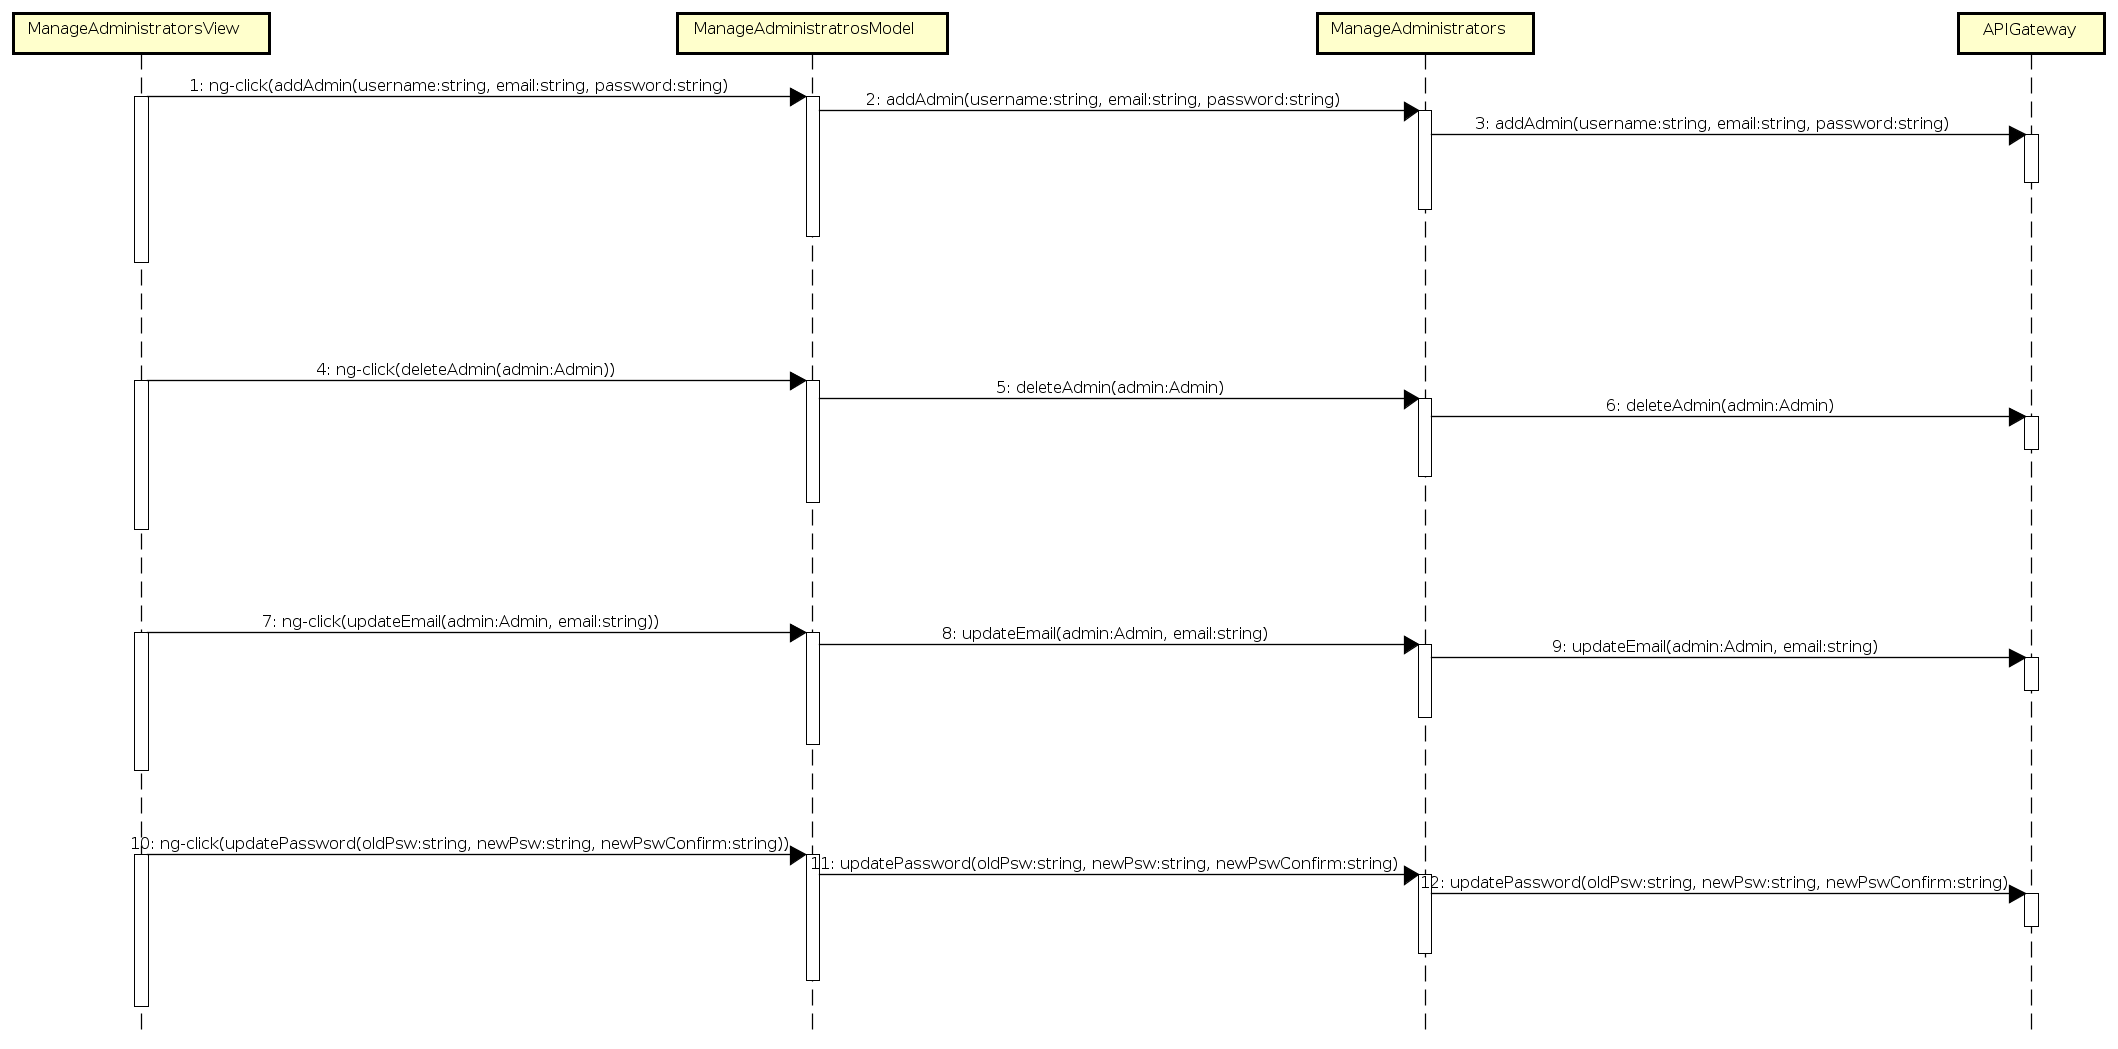
\includegraphics[width=\textwidth]{DiagrammiSequenza/Front-End/AdministrationView/ManageAdministrators.png}
			\caption{Diagramma di sequenza - \texttt{Front-End :: AdministrationView :: AdminComponents :: ManageAdministrators }}
		\end{figure}
		\begin{description}
			\item [Descrizione] Il diagramma di sequenza sopra riportato illustrata l'operazione di gestione degli amministratori da parte del Super amministratore.
			\item [Permessi] Amministratore autenticato.
		\end{description}

		\newpage
		\subsubsection{\texttt{Front-End :: AdministrationView :: AdminComponents :: ManageGuests}}
		\begin{figure}[!h]
			\centering
			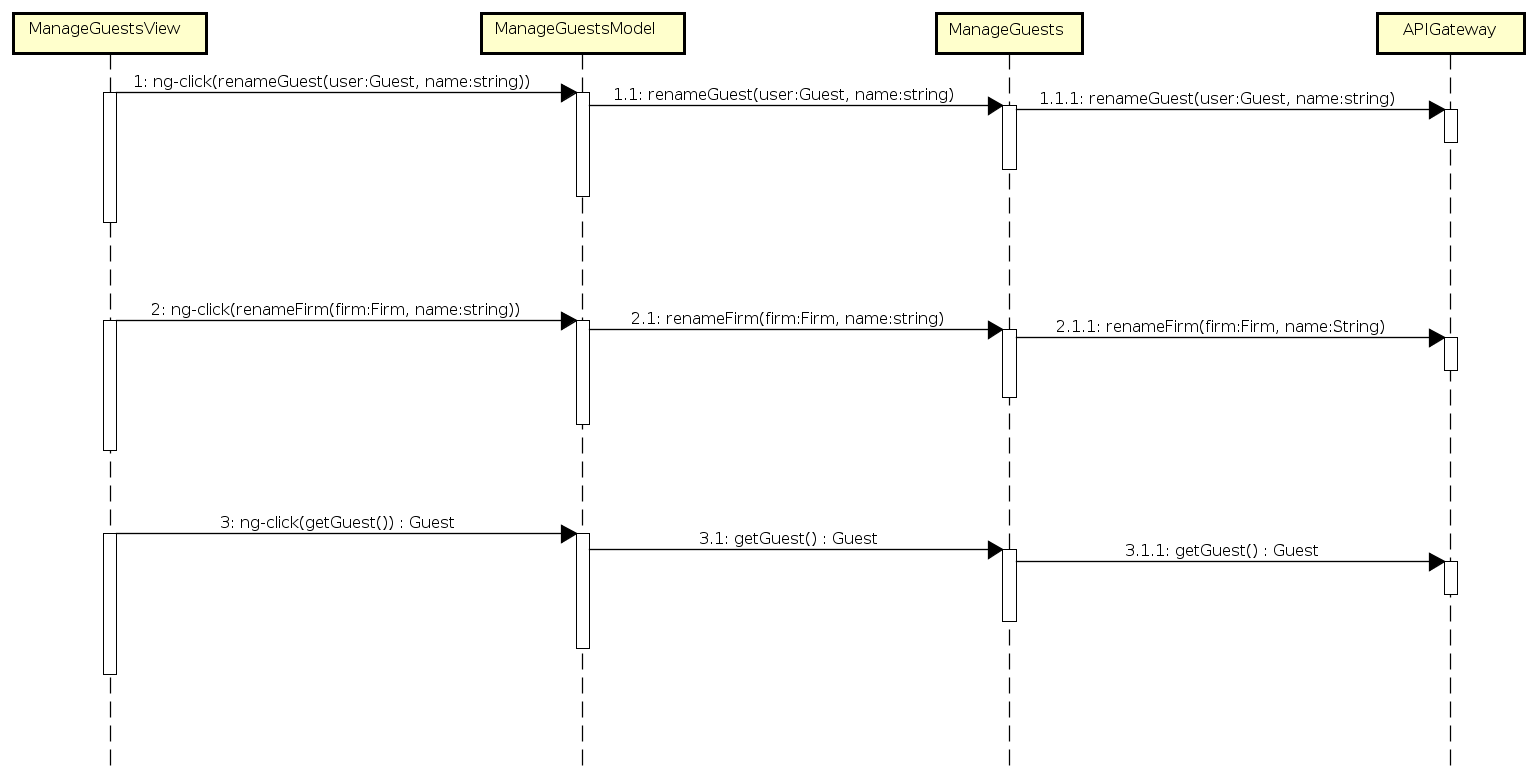
\includegraphics[width=\textwidth]{DiagrammiSequenza/Front-End/AdministrationView/ManageGuests.png}
			\caption{Diagramma di sequenza - \texttt{Front-End :: AdministrationView :: AdminComponents :: ManageGuests }}
		\end{figure}
		\begin{description}
			\item [Descrizione] Il diagramma di sequenza sopra riportato illustra l'operazione di gestione degli ospiti da parte dell'amministratore.
			\item [Permessi] Amministratore autenticato.
		\end{description}

		\subsubsection{\texttt{Front-End :: Administration :: ManageSlack}}
		\begin{figure}[!h]
			\centering
			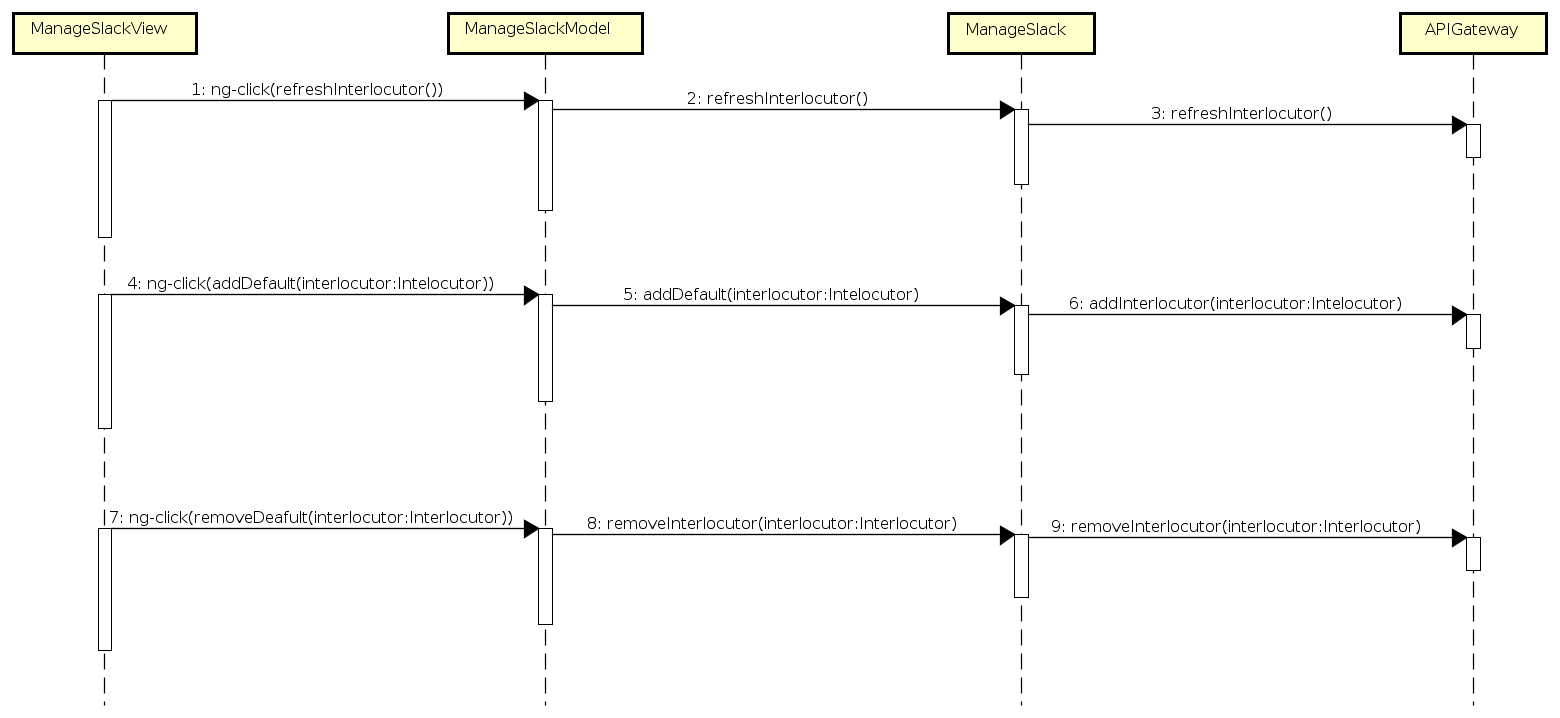
\includegraphics[width=\textwidth]{DiagrammiSequenza/Front-End/AdministrationView/ManageSlack.png}
			\caption{Diagramma di sequenza - \texttt{Front-End :: AdministrationView :: AdminComponents :: ManageSlack }}
		\end{figure}
		\begin{description}
			\item [Descrizione] Il diagramma di sequenza sopra riportato illustra l'operazione di gestione della lista di interlocutori di default da inserire nel canale \#azienda da parte dell'amministratore.
			\item [Permessi] Amministratore autenticato.
		\end{description}

		\subsubsection{\texttt{Front-End :: AdministrationView :: AdminComponents :: ManageQuestions}}
		\begin{figure}[!h]
			\centering
			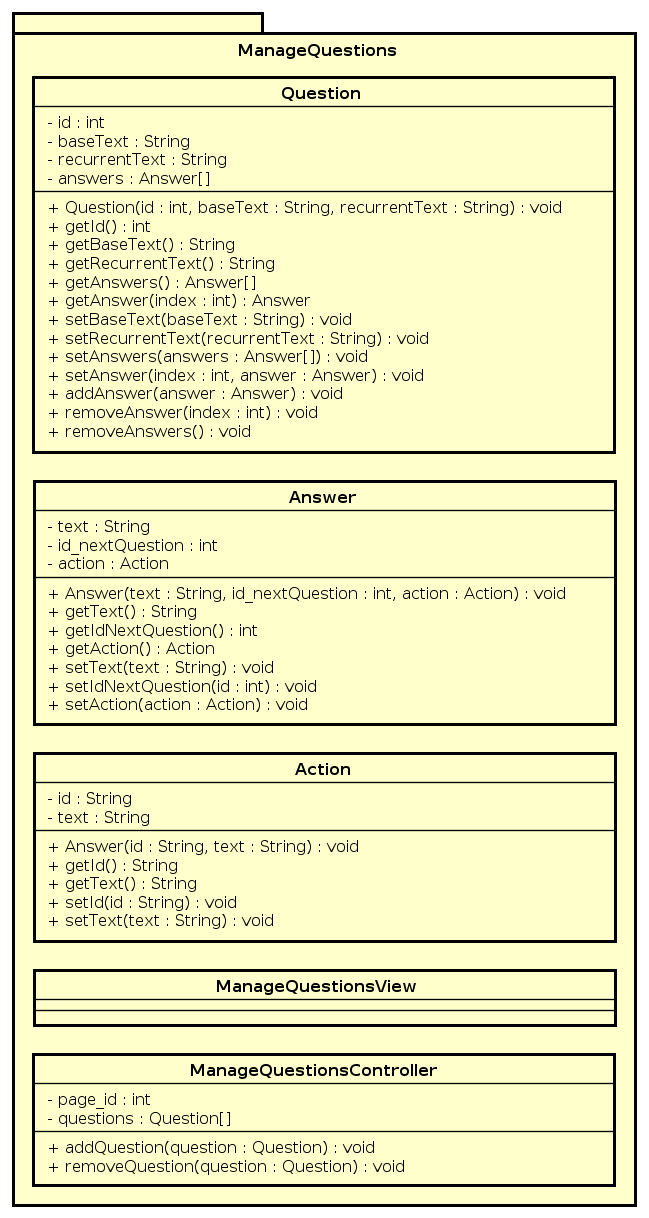
\includegraphics[width=\textwidth]{DiagrammiSequenza/Front-End/AdministrationView/ManageQuestions.png}
			\caption{Diagramma di sequenza - \texttt{Front-End :: AdministrationView :: AdminComponents :: ManageQuestions }}
		\end{figure}
		\begin{description}
			\item [Descrizione] Il diagramma di sequenza sopra riportato illustra l'operazione di gestione delle domande da parte dell'amministratore.
			\item [Permessi] Amministratore autenticato.
		\end{description}

	\subsection{\texttt{Back-End}}
		\subsubsection{\texttt{Guest}}
		\begin{figure}[!h]
			\centering
			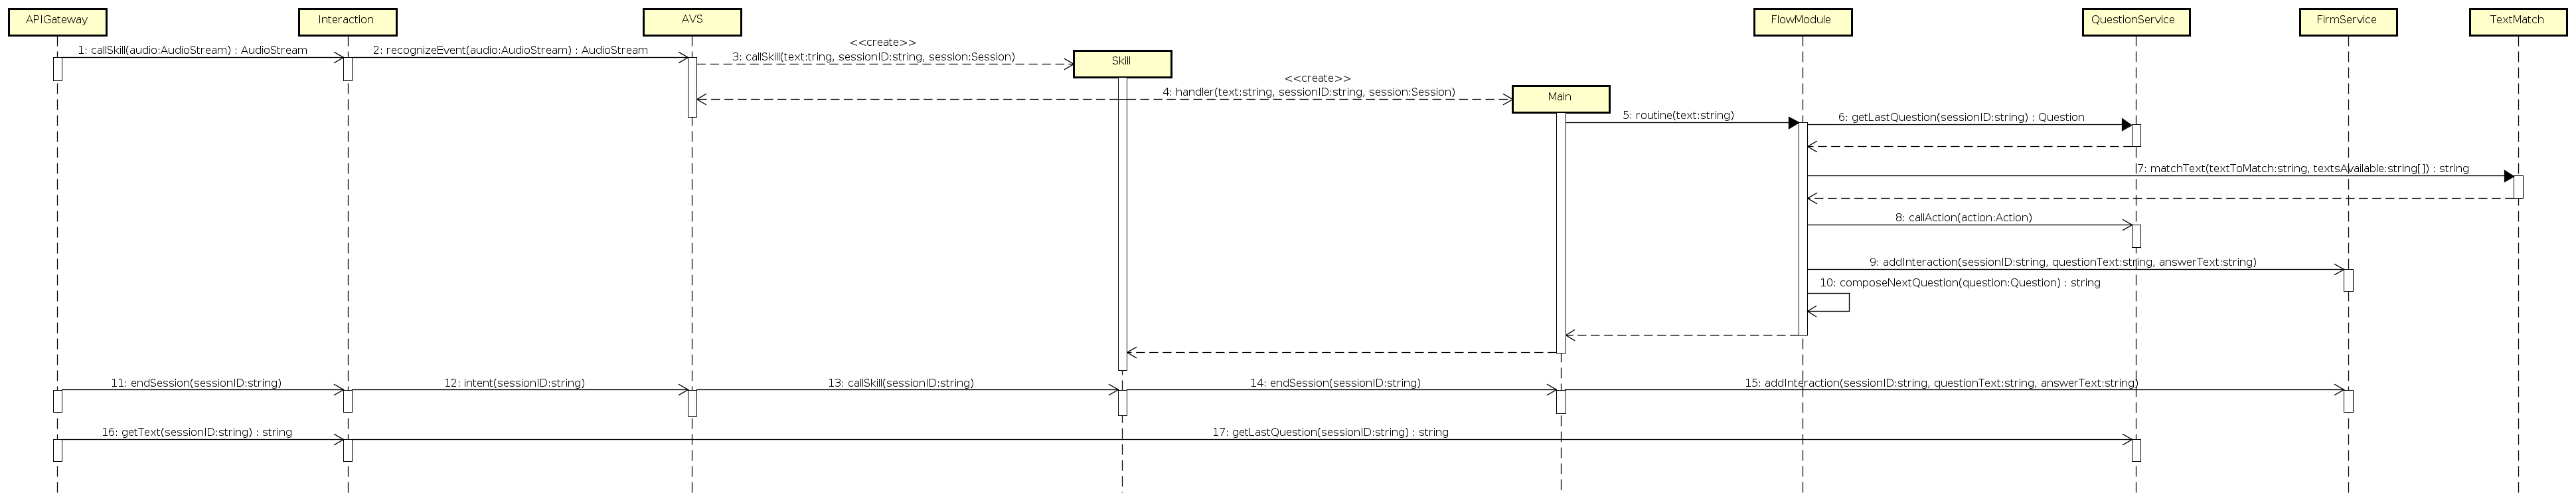
\includegraphics[width=\textwidth]{DiagrammiSequenza/Back-End/DiagrammaSequenzaBackendGuest.png}
			\caption{Diagramma di sequenza - Back-End Guest }
		\end{figure}
		\begin{description}
			\item [Descrizione] Il diagramma di sequenza sopra riportato illustra cosa avviene, in generale, quando viene chiamato un servizio dell'APIGateway per quanto riguarda l'utente Guest.
		\end{description}

		\newpage
		\subsubsection{\texttt{Administrator}}
		\begin{figure}[!h]
			\centering
			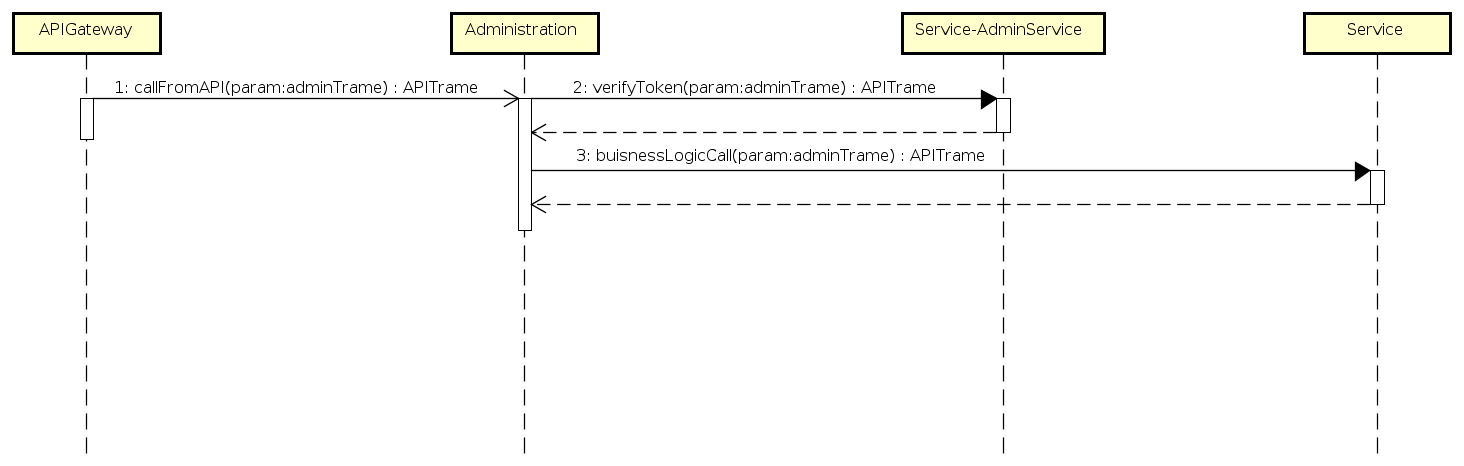
\includegraphics[width=\textwidth]{DiagrammiSequenza/Back-End/DiagrammaSequenzaBackendAdmin.png}
			\caption{Diagramma di sequenza - Back-End Administrator }
		\end{figure}
		\begin{description}
			\item [Descrizione] Il diagramma di sequenza sopra riportato illustra cosa avviene, in generale, quando viene chiamato un servizio dell'APIGateway.
		\end{description}

		\subsubsection{\texttt{Back-End :: Administration :: ManageAdministrators :: addAdmin}}
		\begin{figure}[!h]
			\centering
			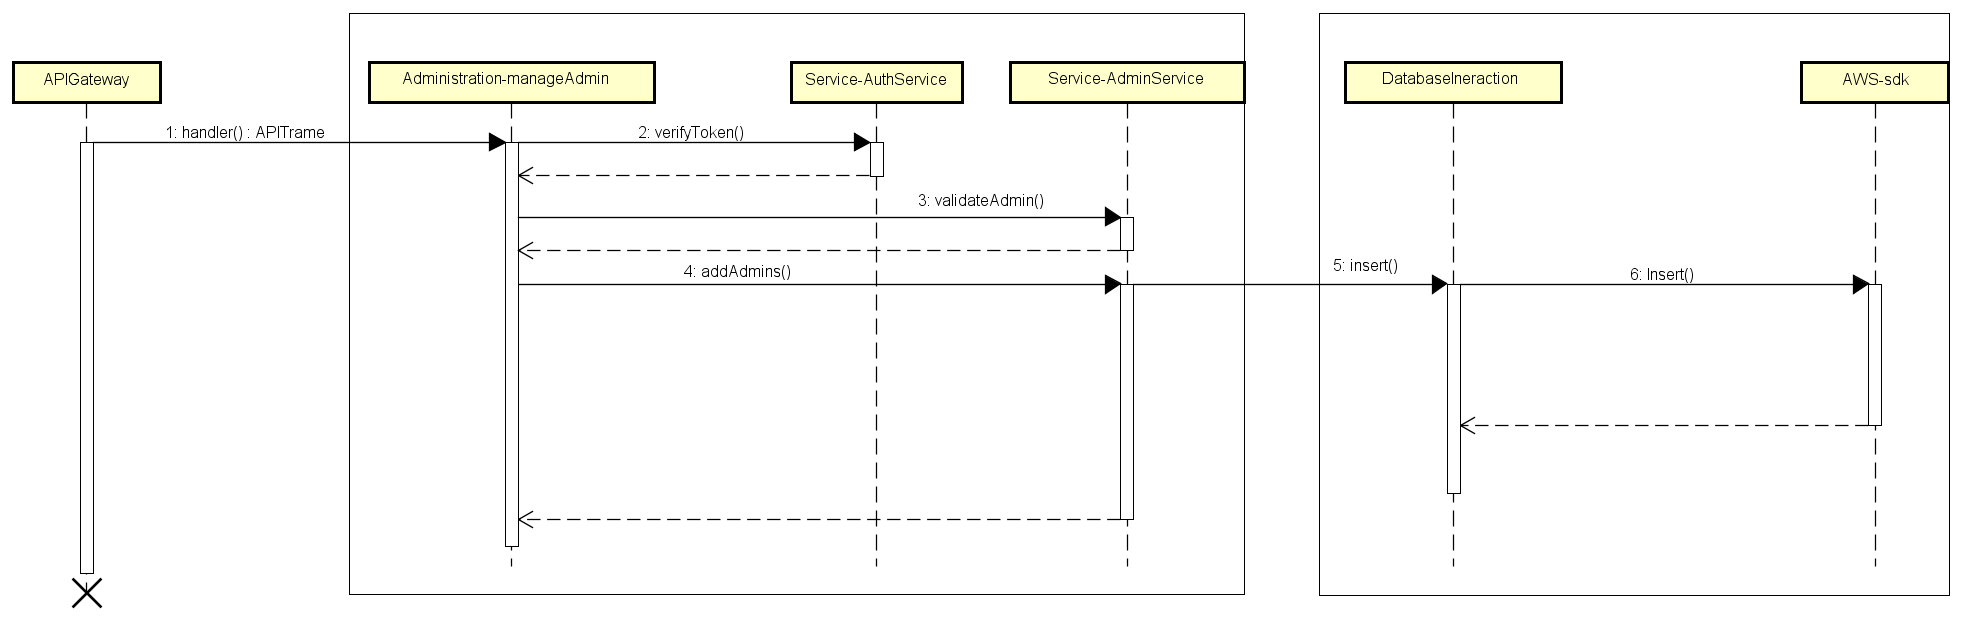
\includegraphics[width=\textwidth]{DiagrammiSequenza/Back-End/manageAdministrators/addAdmin.png}
			\caption{Diagramma di sequenza - \texttt{Back-End :: Administration :: ManageAdministrators :: addAdmin} }
		\end{figure}
		\begin{description}
			\item [Descrizione] Il diagramma di sequenza sopra riportato  llustra la chiamata al servizio addAdmin dell'APIGateway, che permette di aggiungere un nuovo amministratore.
			\item [Permessi] Super Amministratore autenticato.
		\end{description}

		\newpage
		\subsubsection{\texttt{Back-End :: Administration :: ManageAdministrators :: updateAdmin}}
		\begin{figure}[!h]
			\centering
			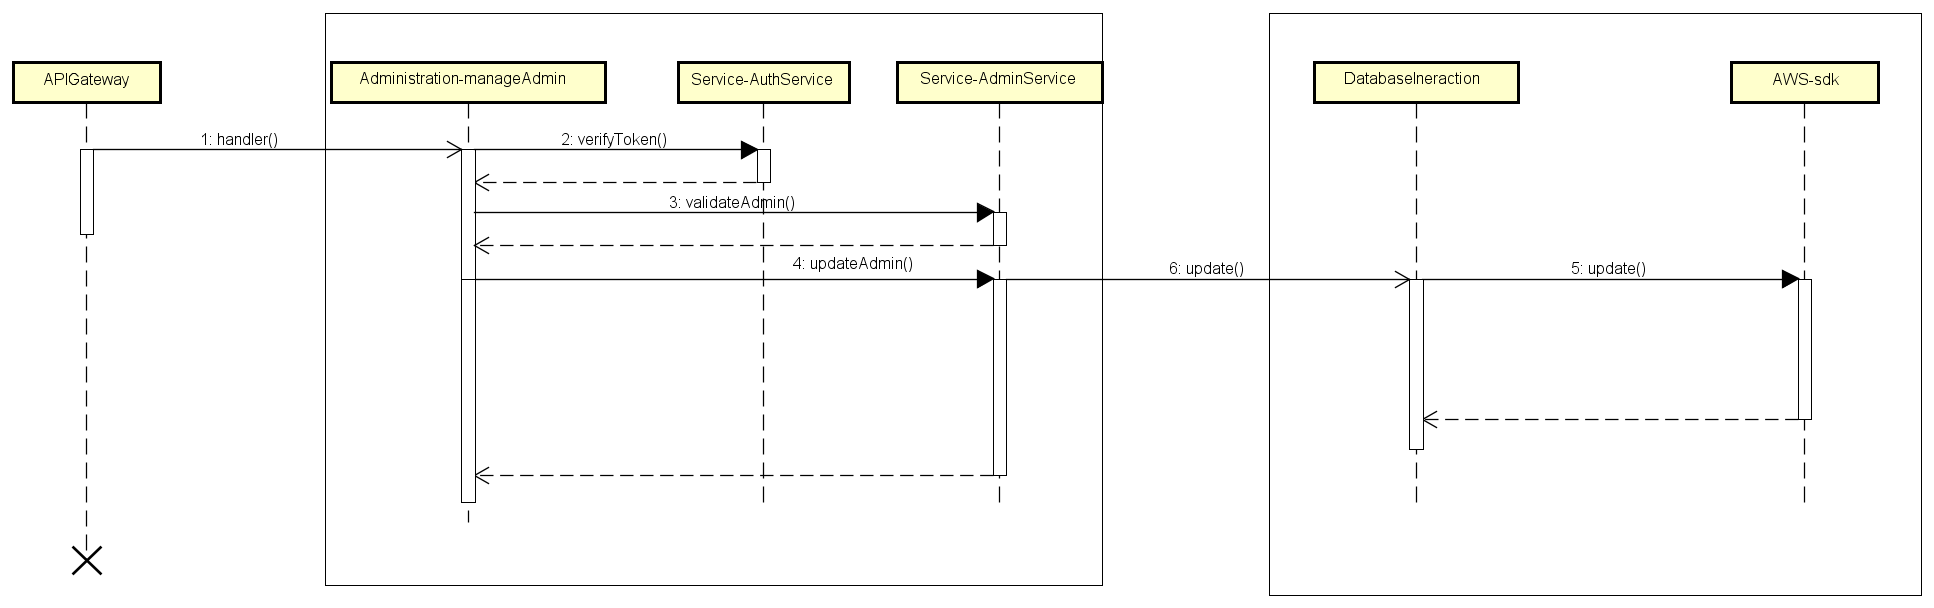
\includegraphics[width=\textwidth]{DiagrammiSequenza/Back-End/manageAdministrators/updateAdmin.png}
			\caption{Diagramma di sequenza - \texttt{Back-End :: Administration :: ManageAdministrators :: updateAdmin }}
		\end{figure}
		\begin{description}
			\item [Descrizione] Il diagramma di sequenza sopra riportato illustra la chiamata al servizio updateAdmin dell'APIGateway, che permette di modificare i dati di un amministratore.
			\item [Permessi] Super Amministratore autenticato.
		\end{description}

		\subsubsection{\texttt{Back-End :: Administration :: ManageAdministrators :: deleteAdmin}}
		\begin{figure}[!h]
			\centering
			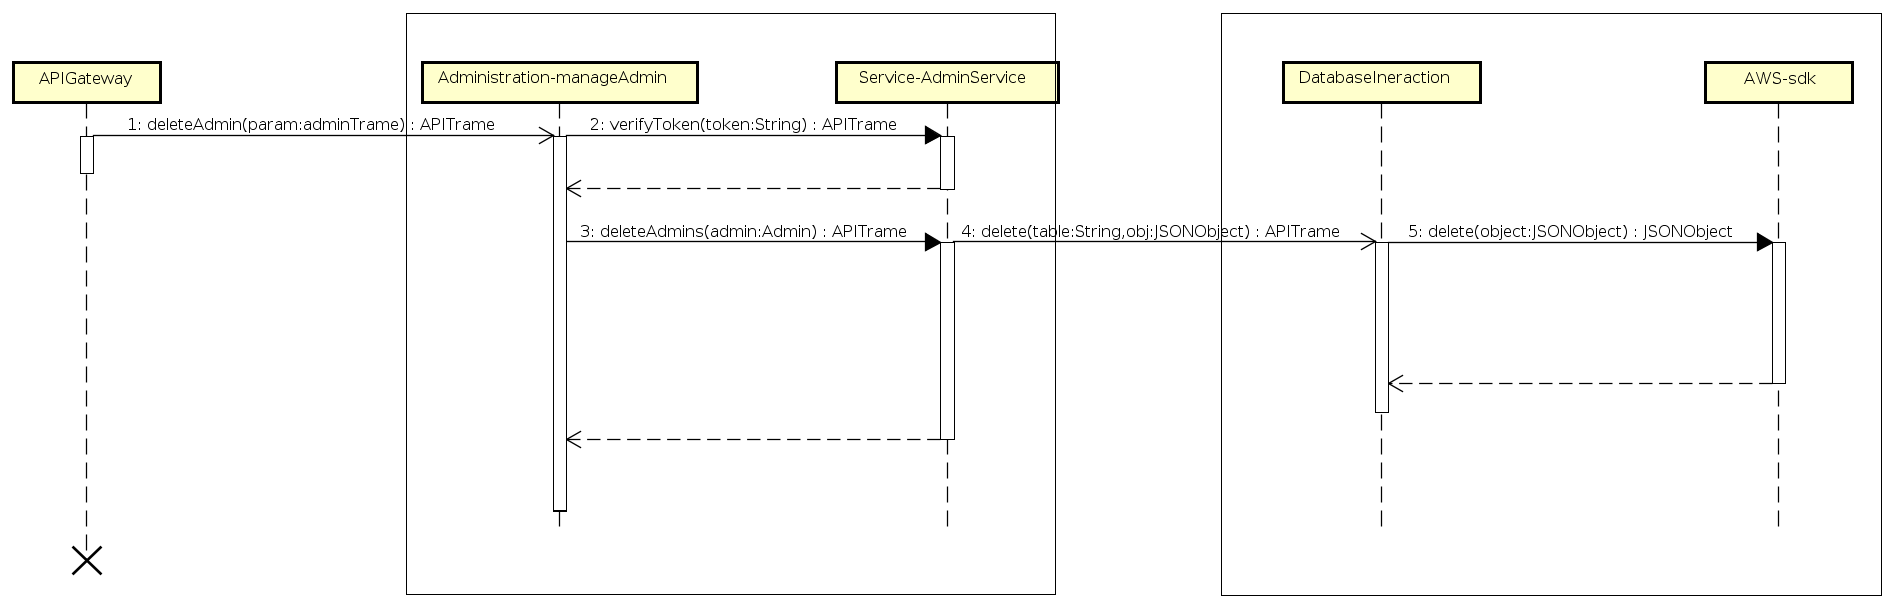
\includegraphics[width=\textwidth]{DiagrammiSequenza/Back-End/manageAdministrators/deleteAdmin.png}
			\caption{Diagramma di sequenza - \texttt{Back-End :: Administration :: ManageAdministrators :: deleteAdmin }}
		\end{figure}
		\begin{description}
			\item [Descrizione] Il diagramma di sequenza sopra riportato illustra la chiamata al servizio deleteAdmin dell'APIGateway, che permette di eliminare un amministratore.
			\item [Permessi] Super Amministratore autenticato.
		\end{description}

		\newpage
		\subsubsection{\texttt{Back-End :: Administration :: ManageAuth :: login}}
		\begin{figure}[!h]
			\centering
			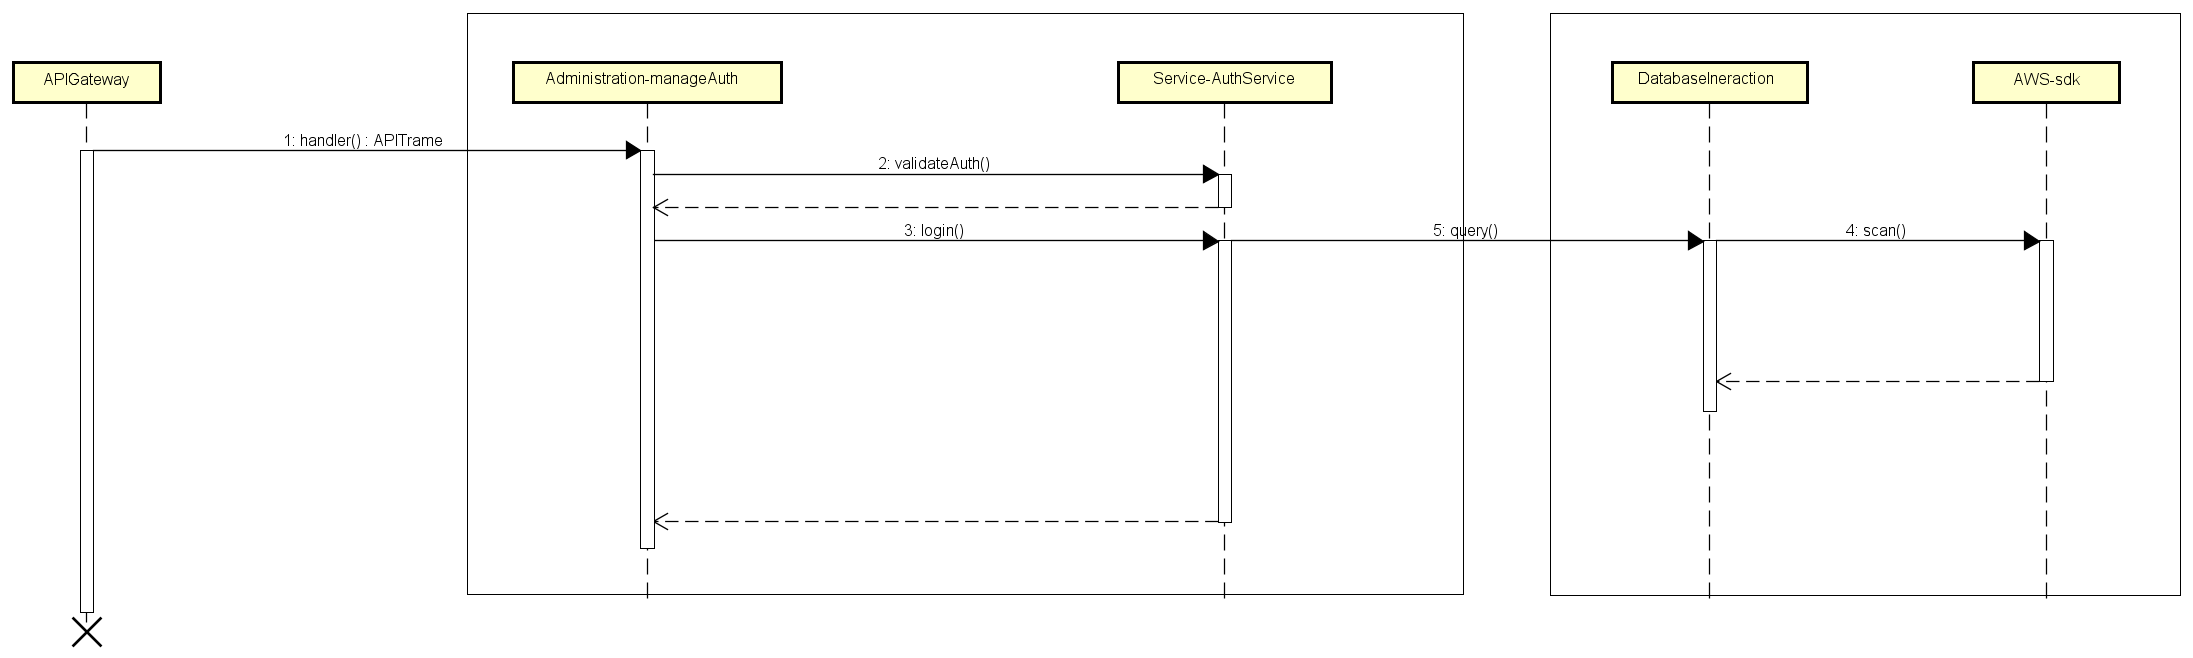
\includegraphics[width=\textwidth]{DiagrammiSequenza/Back-End/manageAuth/login.png}
			\caption{Diagramma di sequenza - \texttt{Back-End :: Administration :: ManageAuth :: login }}
		\end{figure}
		\begin{description}
			\item [Descrizione] Il diagramma di sequenza sopra riportato illustra la chiamata al servizio login dell'APIGateway, che permette di effettuare il login.
			\item [Permessi] Amministratore non autenticato.
		\end{description}

		\subsubsection{\texttt{Back-End :: Administration :: ManageAuth :: logout}}
		\begin{figure}[!h]
			\centering
			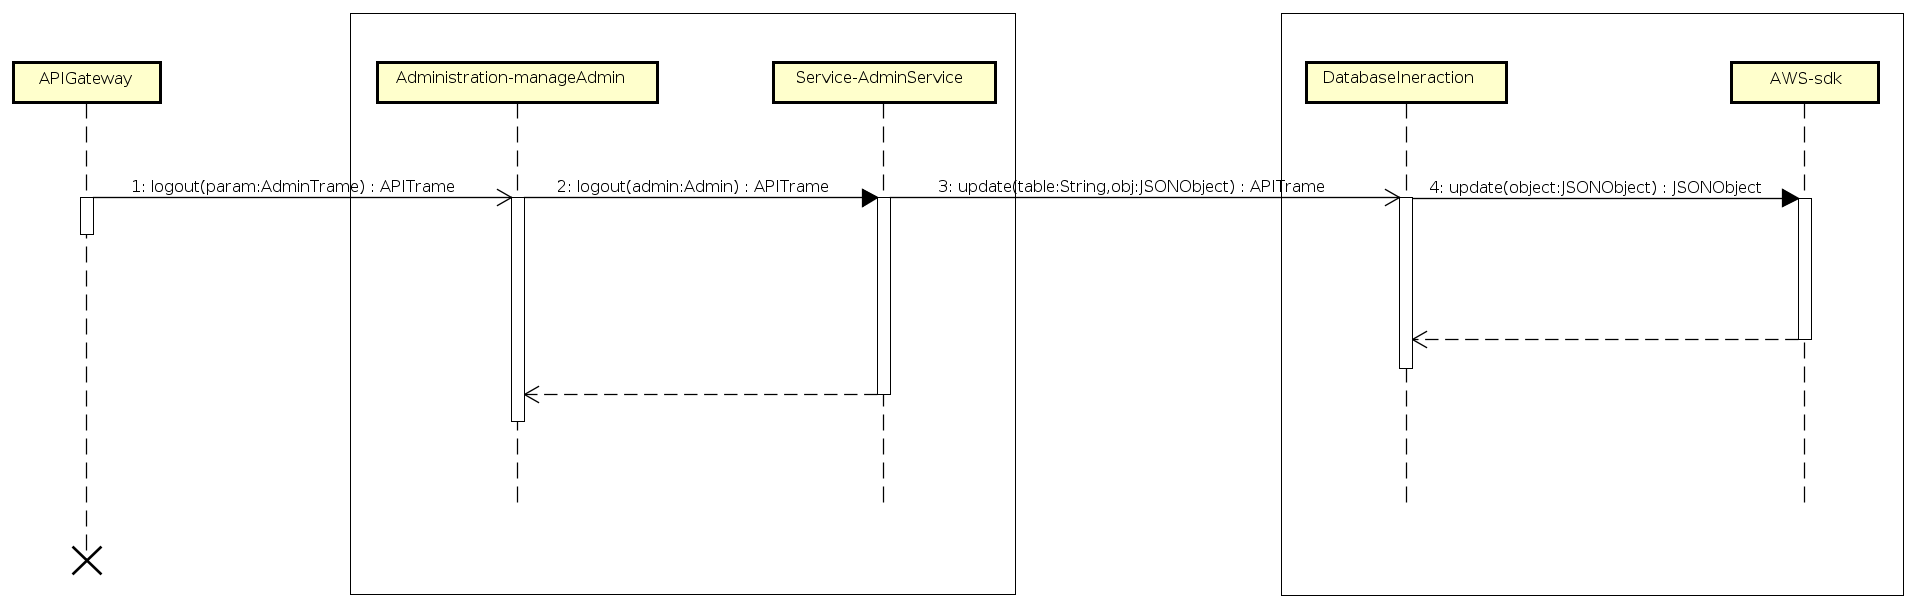
\includegraphics[width=\textwidth]{DiagrammiSequenza/Back-End/manageAuth/logout.png}
			\caption{Diagramma di sequenza - \texttt{Back-End :: Administration :: ManageAuth :: logout }}
		\end{figure}
		\begin{description}
			\item [Descrizione] Il diagramma di sequenza sopra riportato illustra la chiamata al servizio logout dell'APIGateway, che permette di deautenticare un amministratore.
			\item [Permessi] Amministratore autenticato.
		\end{description}

		\newpage
		\subsubsection{\texttt{Back-End :: Administration :: ManageAuth :: sendEmail}}
		\begin{figure}[!h]
			\centering
			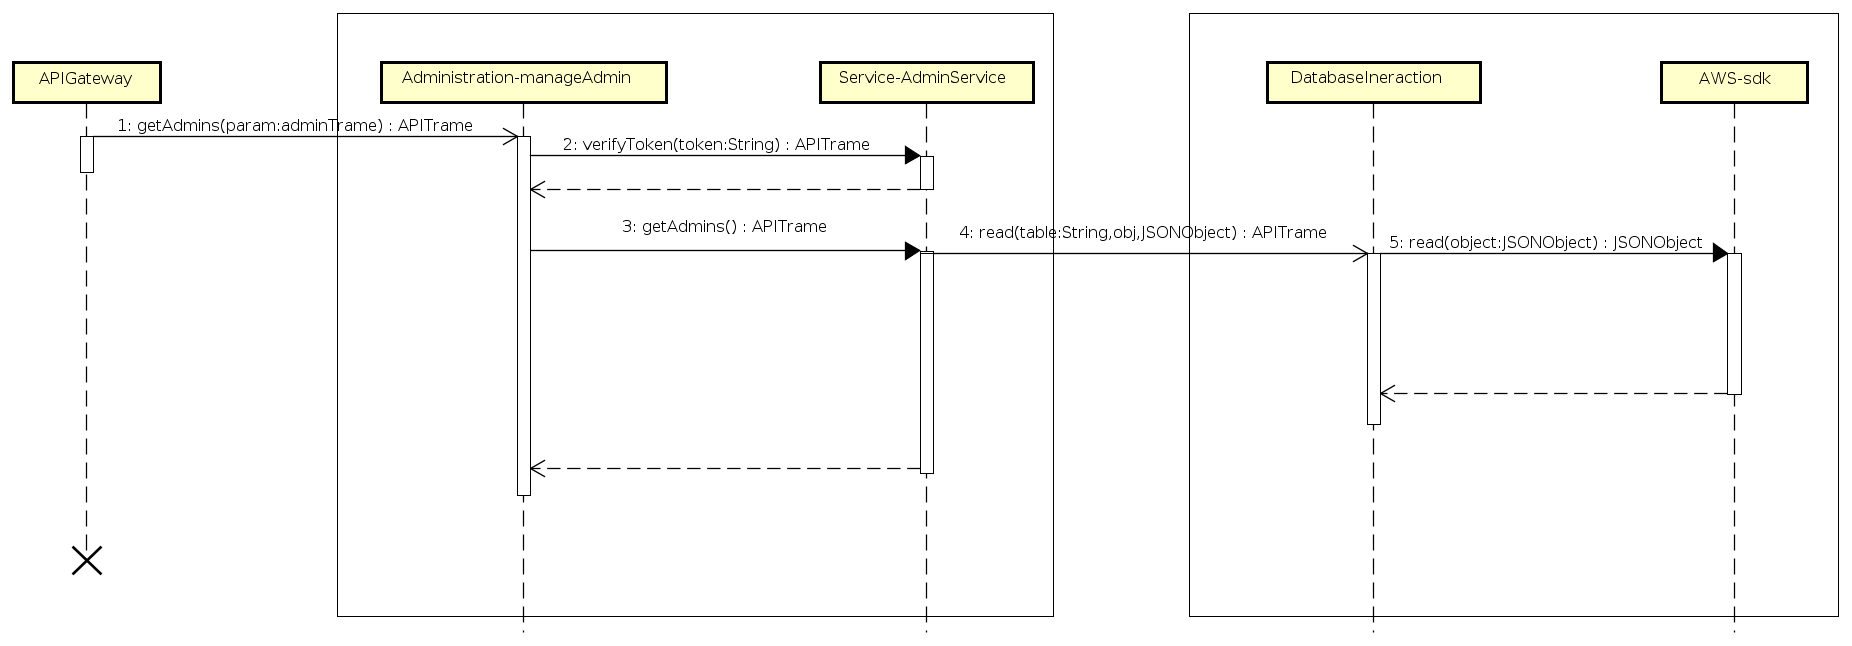
\includegraphics[width=\textwidth]{DiagrammiSequenza/Back-End/manageAuth/sendEmail.png}
			\caption{Diagramma di sequenza - \texttt{Back-End :: Administration :: ManageAuth :: sendEmail }}
		\end{figure}
		\begin{description}
			\item [Descrizione] Il diagramma di sequenza sopra riportato illustra la chiamata al servizio sendEmail dell'APIGateway, che permette di inviare una mail per il recupero della password ad un amministratore.
			\item [Permessi] Amministratore non autenticato.
		\end{description}

		\subsubsection{\texttt{Back-End :: Administration :: ManageAuth :: verifyLogin}}
		\begin{figure}[!h]
			\centering
			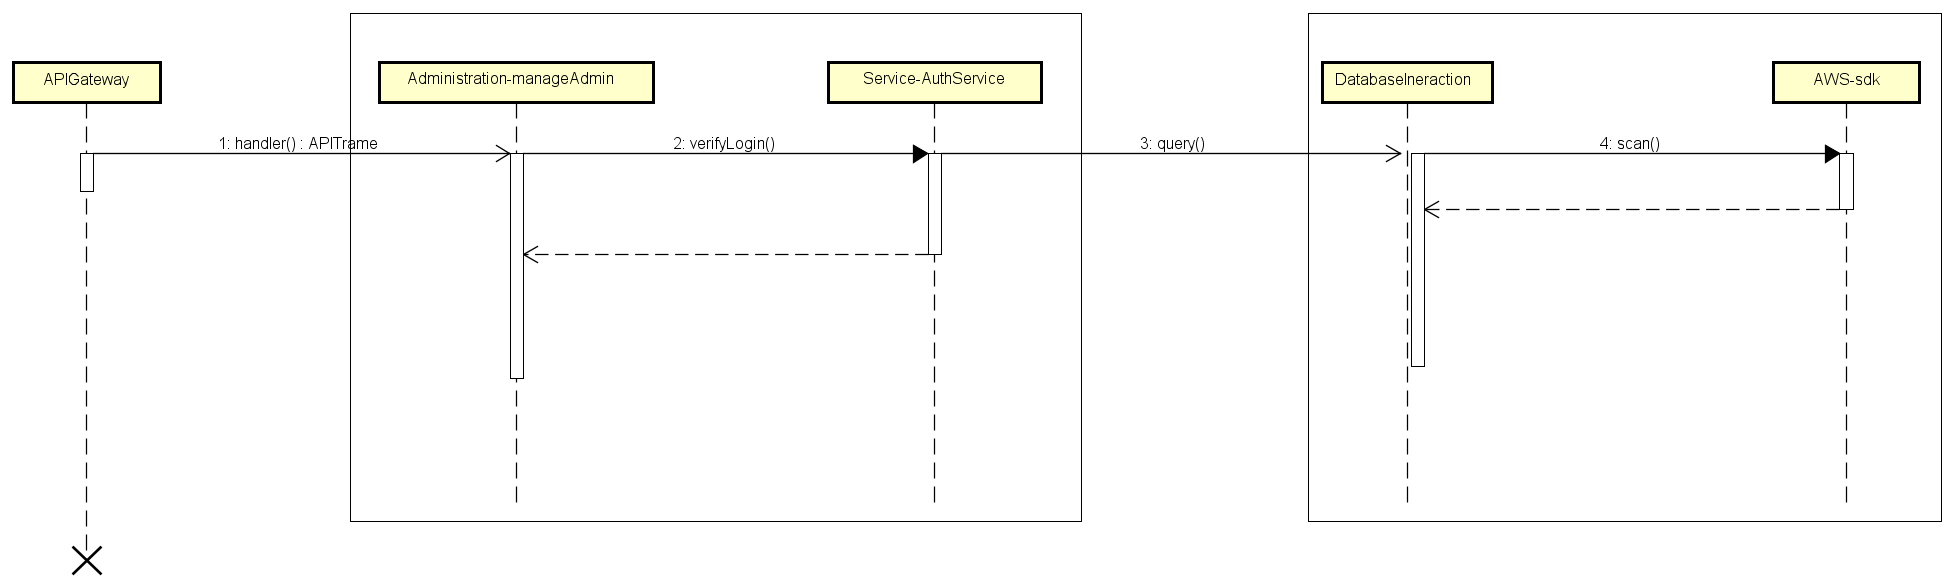
\includegraphics[width=\textwidth]{DiagrammiSequenza/Back-End/manageAuth/verifyLogin.png}
			\caption{Diagramma di sequenza - \texttt{Back-End :: Administration :: ManageAuth :: verifyLogin }}
		\end{figure}
		\begin{description}
			\item [Descrizione] Il diagramma di sequenza sopra riportato illustra la chiamata al servizio verifyLogin dell'APIGateway, che permette di verificare che il token di login dell'utente sia autentico.
			\item [Permessi] Amministratore autenticato.
		\end{description}

		\newpage
		\subsubsection{\texttt{Back-End :: Administration :: ManageFirm :: getFirms}}
		\begin{figure}[!h]
			\centering
			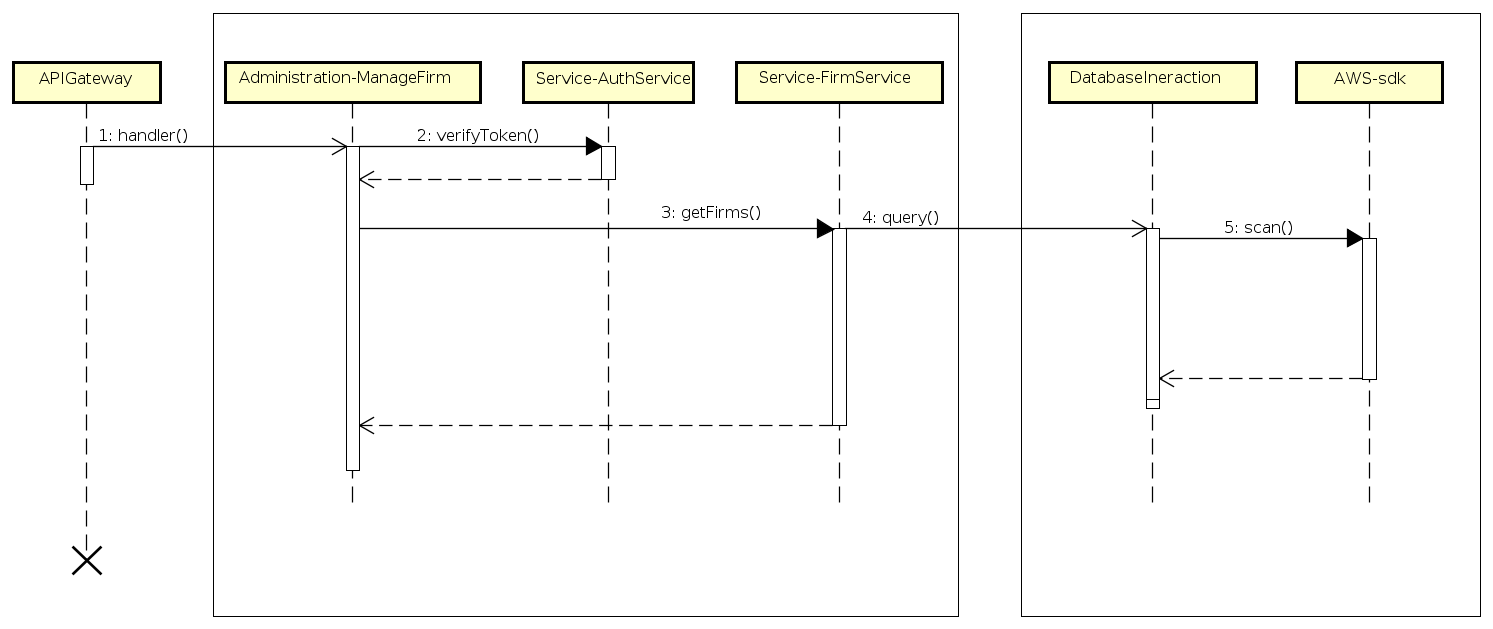
\includegraphics[width=\textwidth]{DiagrammiSequenza/Back-End/manageFirm/getFirms.png}
			\caption{Diagramma di sequenza - \texttt{Back-End :: Administration :: ManageFirm :: getFirms }}
		\end{figure}
		\begin{description}
			\item [Descrizione] Il diagramma di sequenza sopra riportato illustra la chiamata al servizio getFirms dell'APIGateway, che permette di ottenere la lista delle aziende.
			\item [Permessi] Amministratore autenticato.
		\end{description}

		\subsubsection{\texttt{Back-End :: Administration :: ManageFirm :: updateFirm}}
		\begin{figure}[!h]
			\centering
			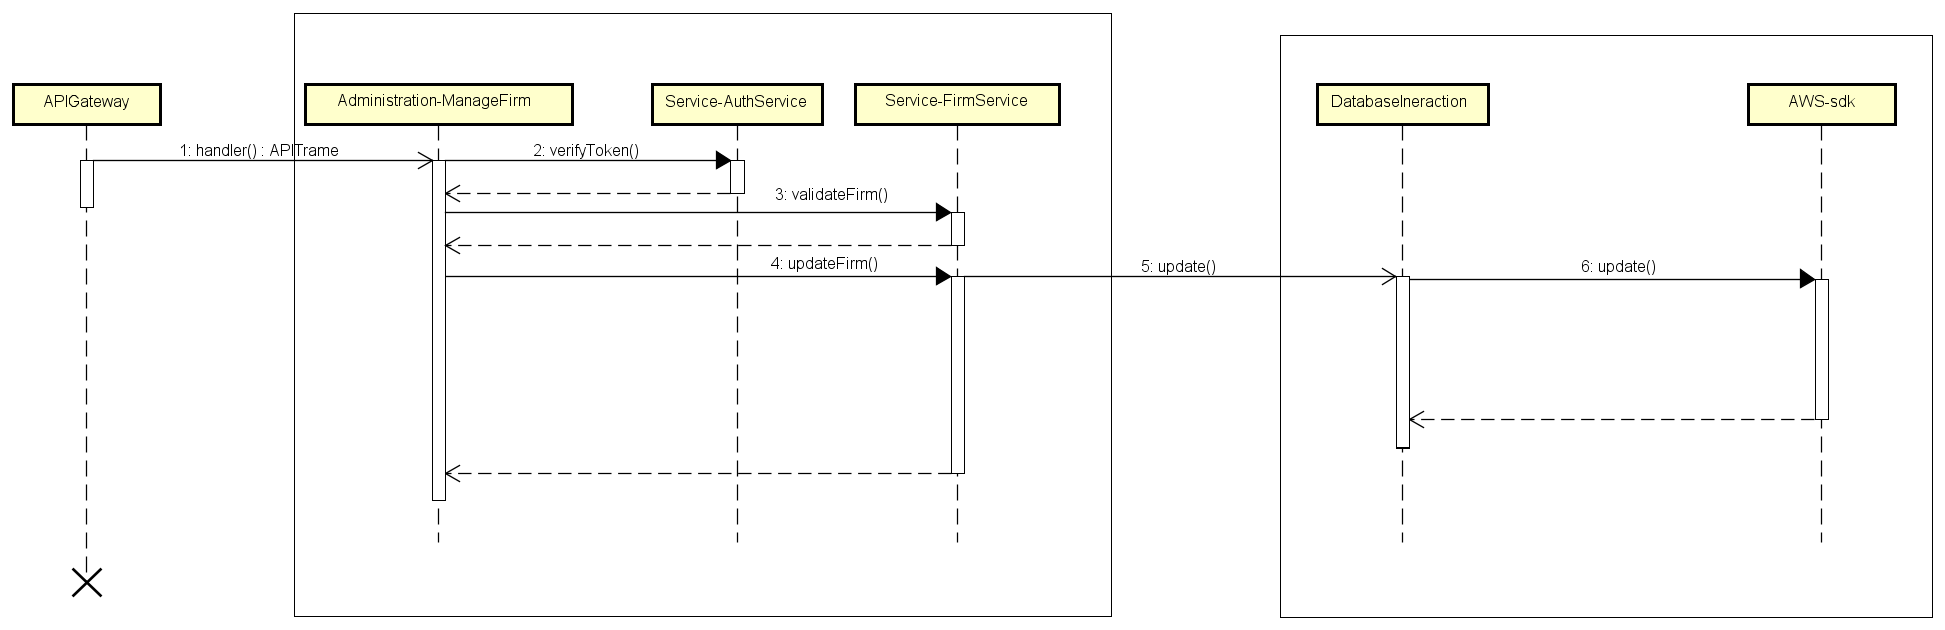
\includegraphics[width=\textwidth]{DiagrammiSequenza/Back-End/manageFirm/updateFirm.png}
			\caption{Diagramma di sequenza - \texttt{Back-End :: Administration :: ManageFirm :: updateFirm }}
		\end{figure}
		\begin{description}
			\item [Descrizione] Il diagramma di sequenza sopra riportato illustra la chiamata al servizio updateFirm dell'APIGateway, che permette di modificare i dati di un azienda.
			\item [Permessi] Amministratore autenticato.
		\end{description}

		\newpage
		\subsubsection{\texttt{Back-End :: Administration :: ManageFirm :: getGuestConversation}}
		\begin{figure}[!h]
			\centering
			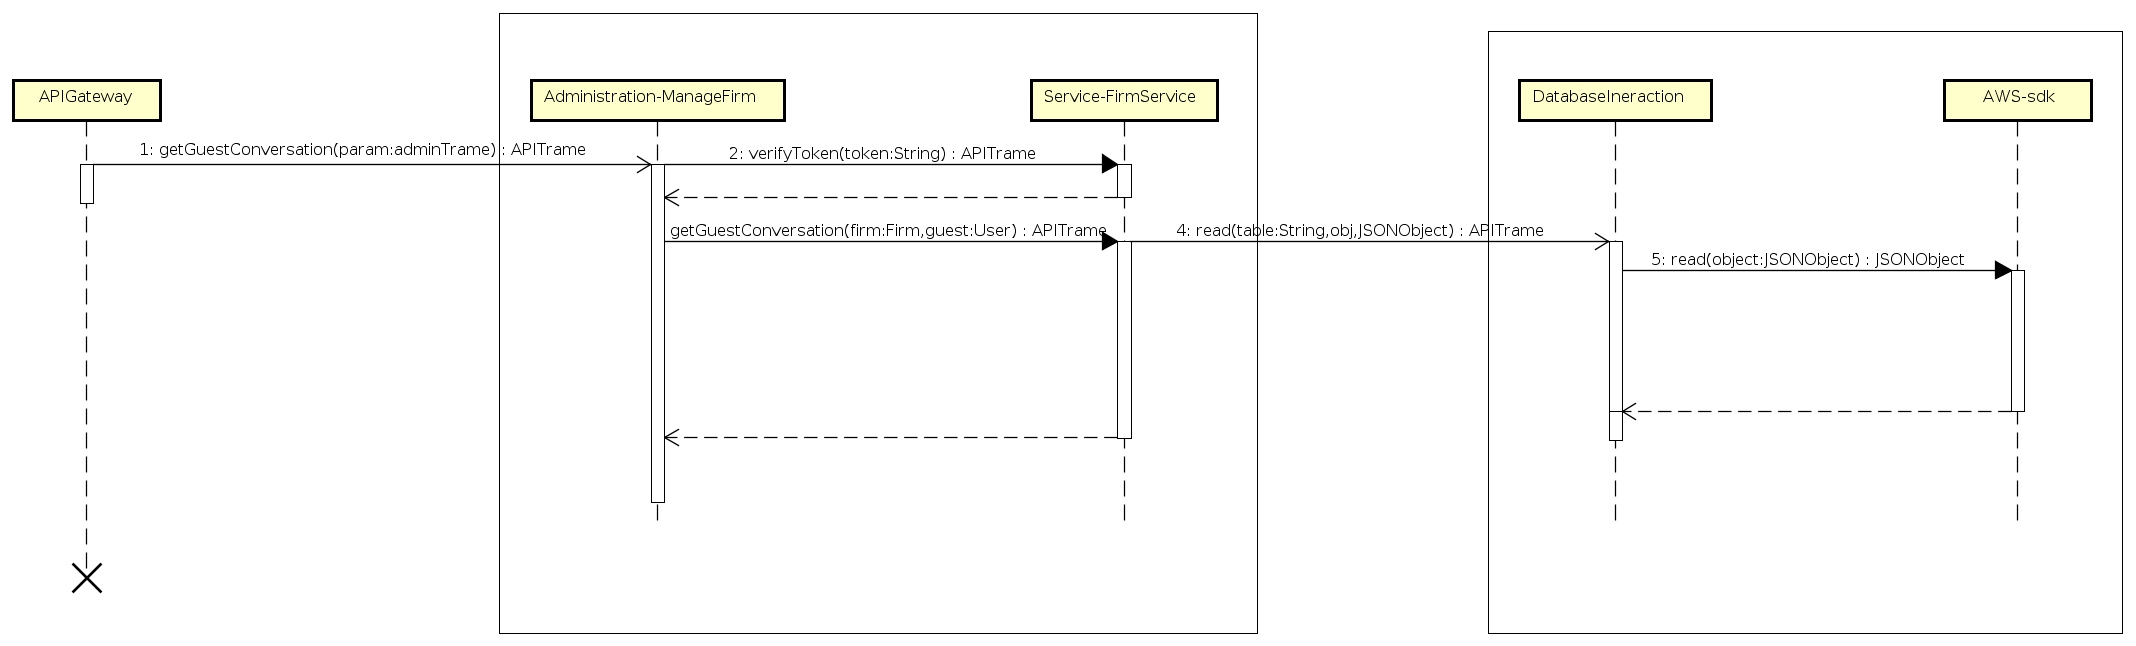
\includegraphics[width=\textwidth]{DiagrammiSequenza/Back-End/manageFirm/getGuestConversation.png}
			\caption{Diagramma di sequenza - \texttt{Back-End :: Administration :: ManageFirm :: getGuestConversation }}
		\end{figure}
		\begin{description}
			\item [Descrizione] Il diagramma di sequenza sopra riportato illustra la chiamata al servizio getGuestConversation dell'APIGateway, che permette di ottenere le conversazioni di un ospite.
			\item [Permessi] Amministratore autenticato.
		\end{description}

		\subsubsection{\texttt{Back-End :: Administration :: ManageQuestion :: addQuestion}}
		\begin{figure}[!h]
			\centering
			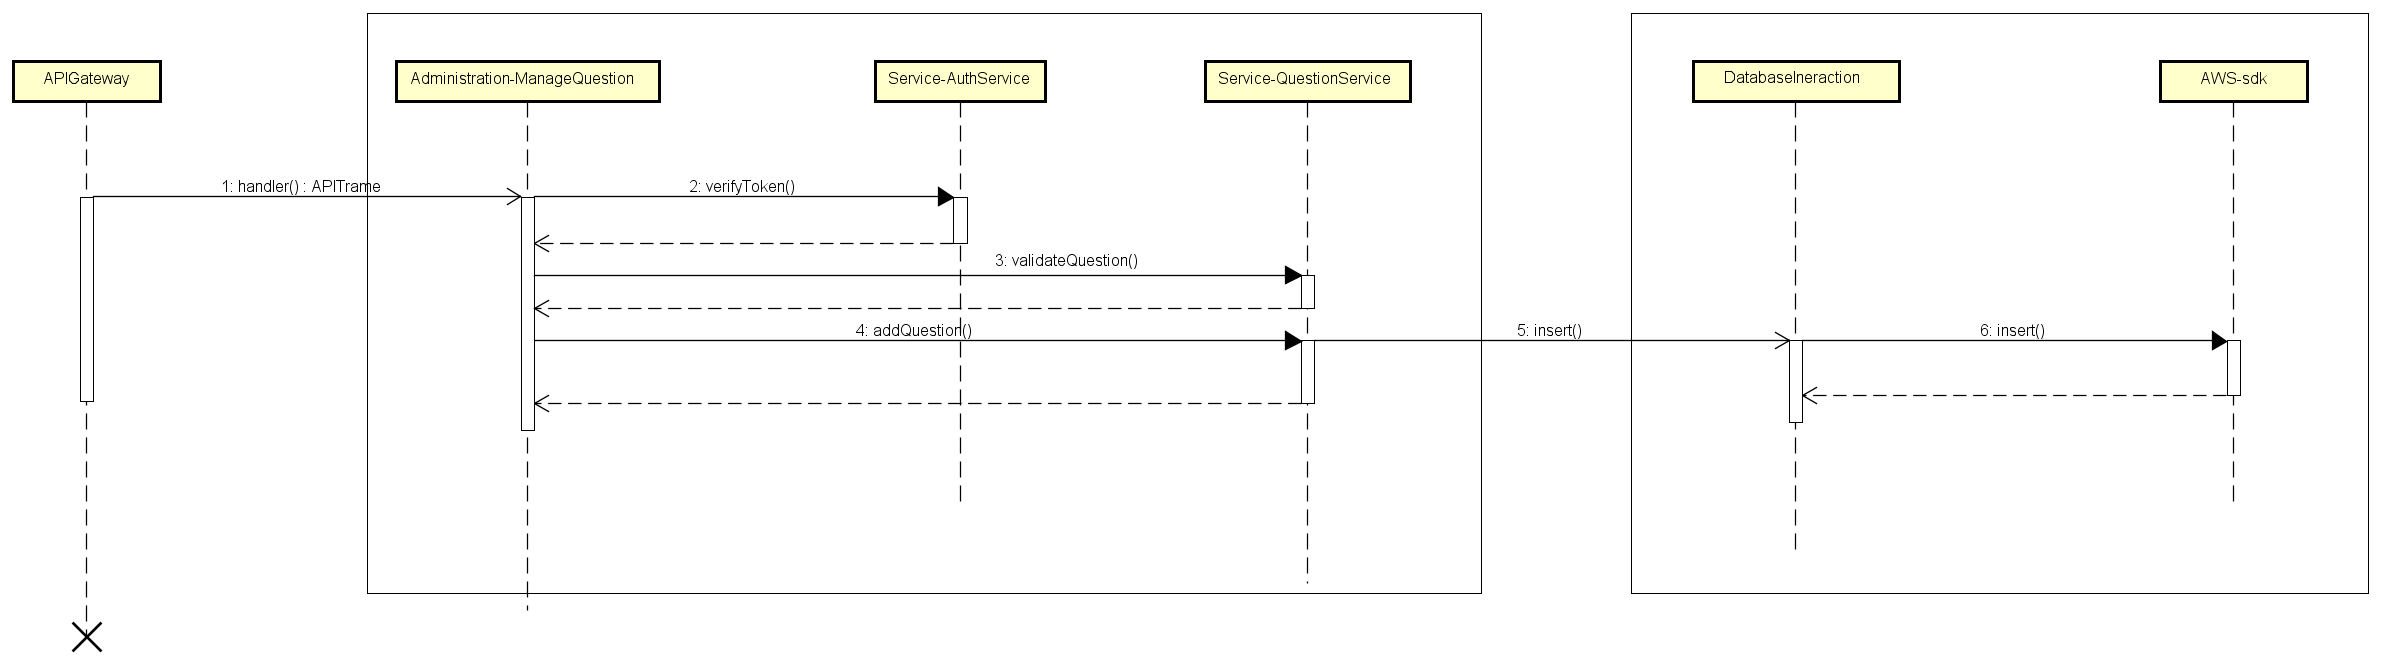
\includegraphics[width=\textwidth]{DiagrammiSequenza/Back-End/manageQuestion/addQuestion.png}
			\caption{Diagramma di sequenza - \texttt{Back-End :: Administration :: ManageQuestion :: addQuestion }}
		\end{figure}
		\begin{description}
			\item [Descrizione] Il diagramma di sequenza sopra riportato illustra la chiamata al servizio addQuestion dell'APIGateway, che permette di aggiungere una domanda.
			\item [Permessi] Amministratore autenticato.
		\end{description}

		\newpage
		\subsubsection{\texttt{Back-End :: Administration :: ManageQuestion :: deleteQuestion}}
		\begin{figure}[!h]
			\centering
			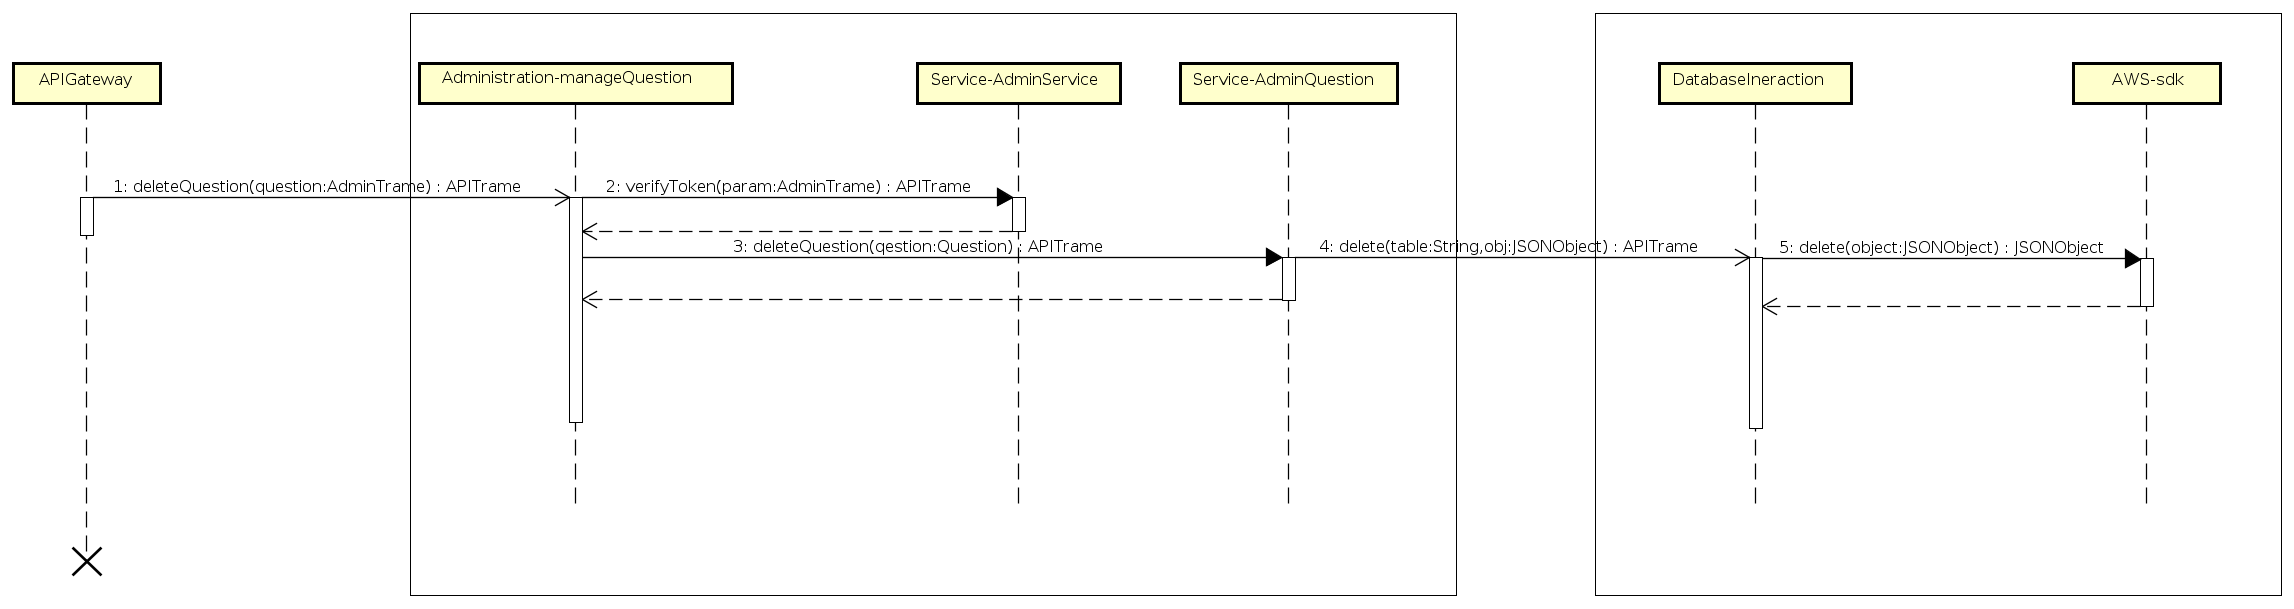
\includegraphics[width=\textwidth]{DiagrammiSequenza/Back-End/manageQuestion/deleteQuestion.png}
			\caption{Diagramma di sequenza - \texttt{Back-End :: Administration :: ManageQuestion :: deleteQuestion }}
		\end{figure}
		\begin{description}
			\item [Descrizione] Il diagramma di sequenza sopra riportato  llustra la chiamata al servizio deleteQuestion dell'APIGateway, che permette di eliminare una risposta.
			\item [Permessi] Amministratore autenticato.
		\end{description}

		\subsubsection{\texttt{Back-End :: Administration :: ManageQuestion :: getAction}}
		\begin{figure}[!h]
			\centering
			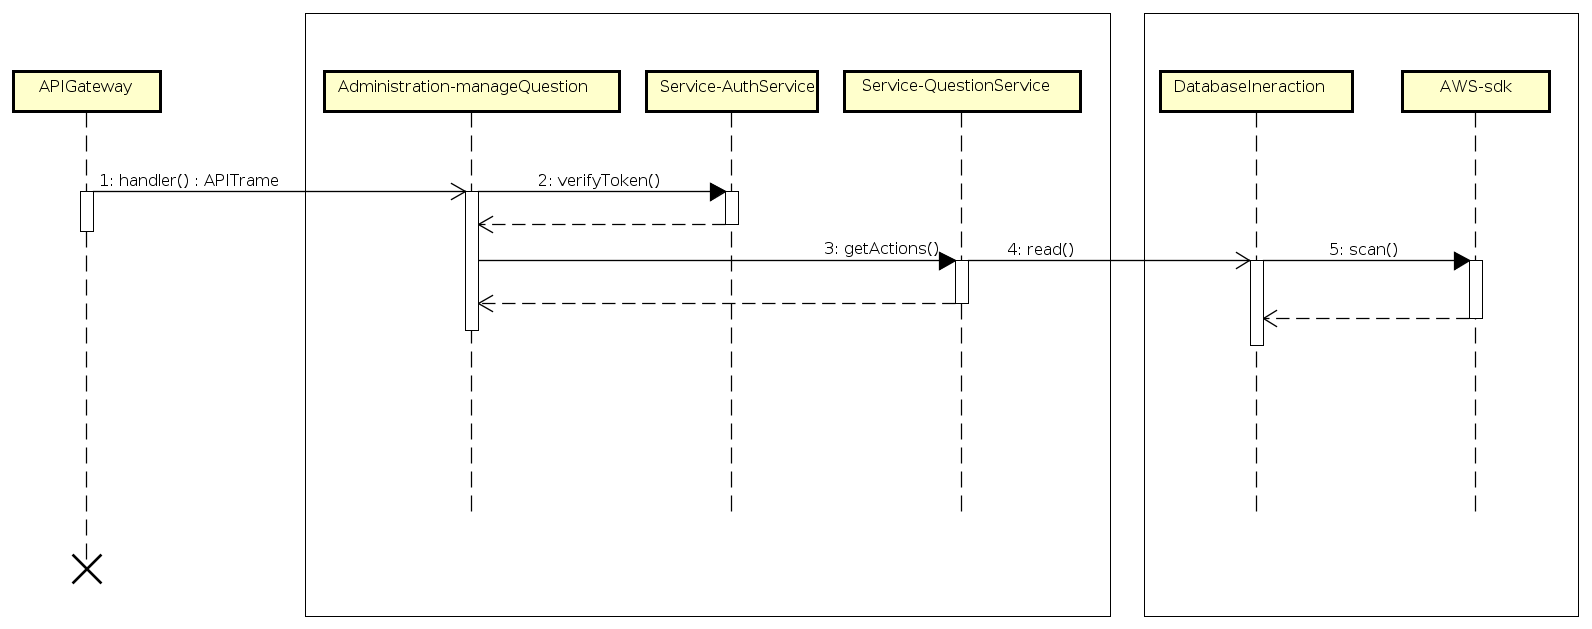
\includegraphics[width=\textwidth]{DiagrammiSequenza/Back-End/manageQuestion/getAction.png}
			\caption{Diagramma di sequenza - \texttt{Back-End :: Administration :: ManageQuestion :: getAction} }
		\end{figure}
		\begin{description}
			\item [Descrizione] Il diagramma di sequenza sopra riportato illustra la chiamata al servizio getAction dell'APIGateway, che permette di ottenere l'azione legata ad una risposta.
			\item [Permessi] Amministratore autenticato.
		\end{description}

		\newpage
		\subsubsection{\texttt{Back-End :: Administration :: ManageQuestion :: getQuestions}}
		\begin{figure}[!h]
			\centering
			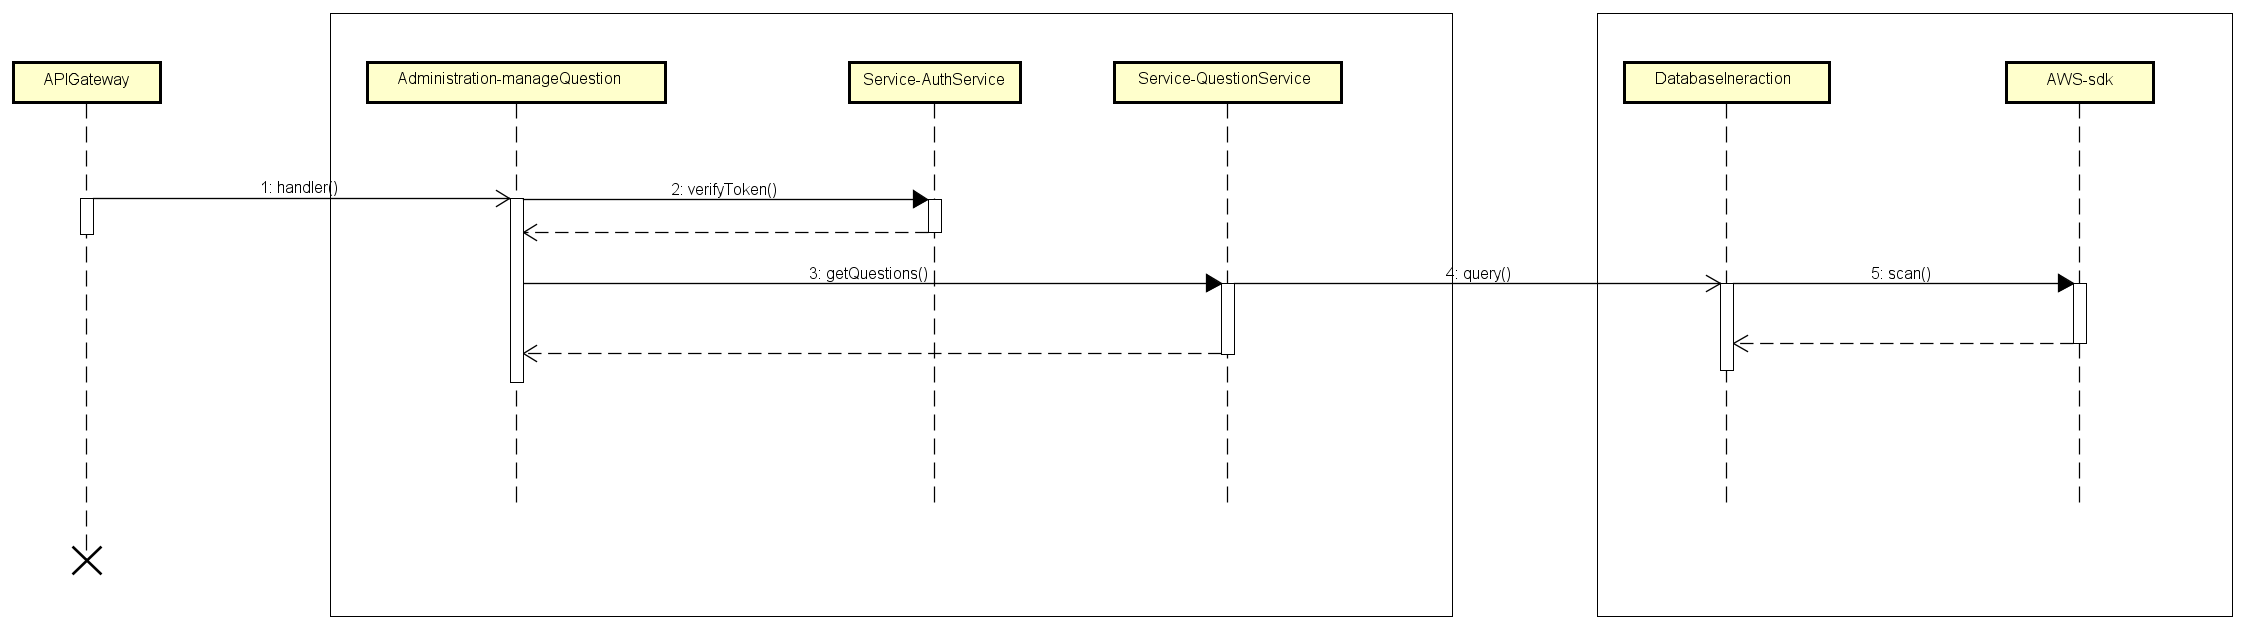
\includegraphics[width=\textwidth]{DiagrammiSequenza/Back-End/manageQuestion/getQuestion.png}
			\caption{Diagramma di sequenza - \texttt{Back-End :: Administration :: ManageQuestion :: getQuestions }}
		\end{figure}
		\begin{description}
			\item [Descrizione] Il diagramma di sequenza sopra riportato illustra la chiamata al servizio getQuestion dell'APIGateway, che permette di ottenere la lista delle domande.
			\item [Permessi] Amministratore autenticato.
		\end{description}

		\subsubsection{\texttt{Back-End :: Administration :: ManageQuestion :: updateQuestion}}
		\begin{figure}[!h]
			\centering
			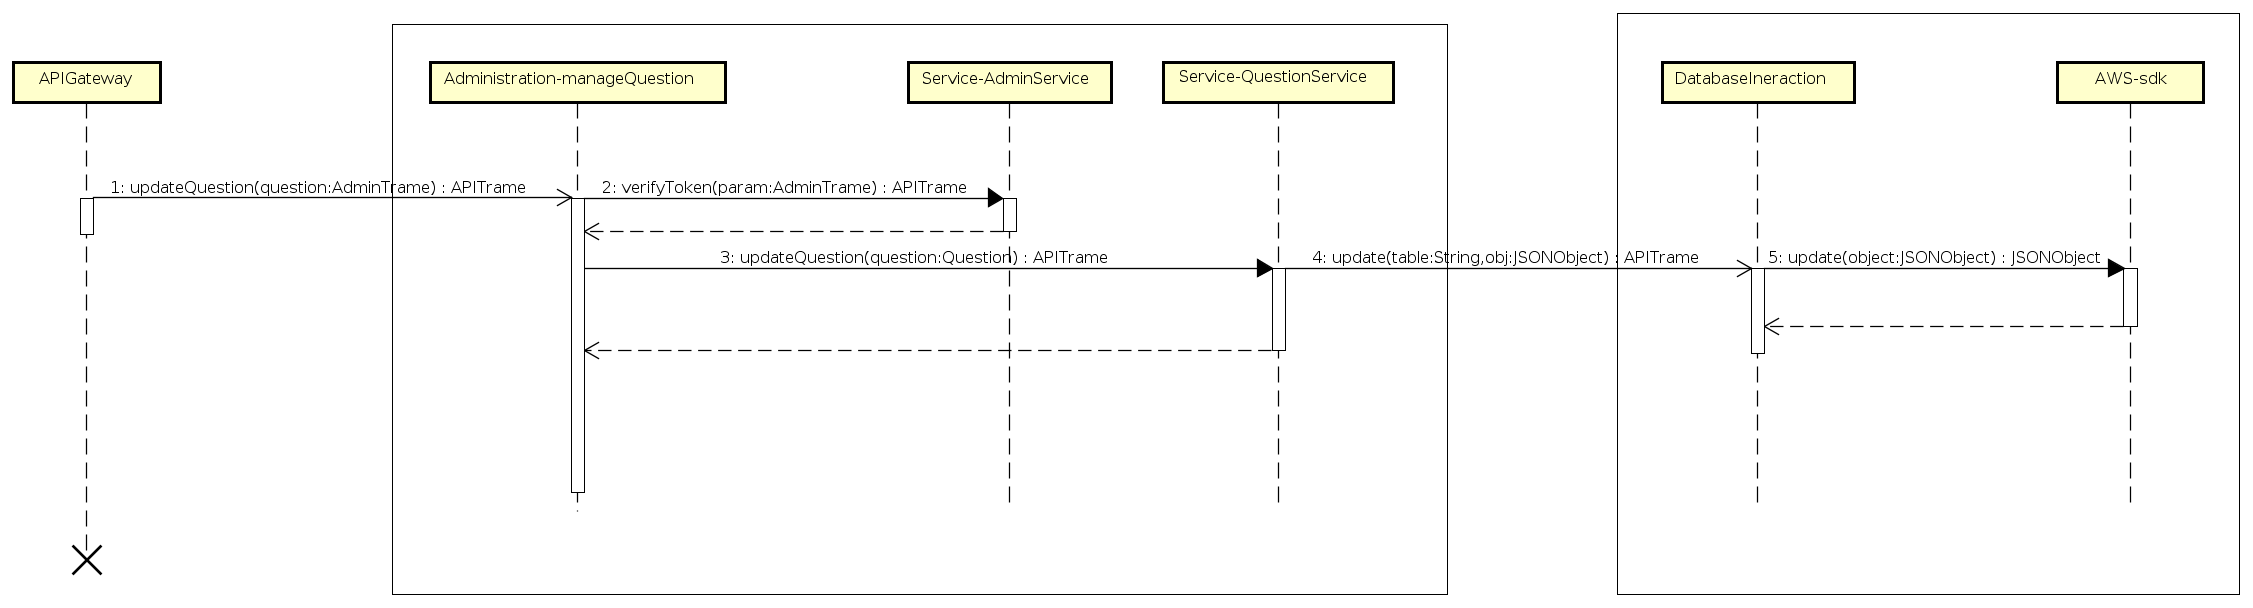
\includegraphics[width=\textwidth]{DiagrammiSequenza/Back-End/manageQuestion/updateQuestion.png}
			\caption{Diagramma di sequenza - \texttt{Back-End :: Administration :: ManageQuestion :: updateQuestion} }
		\end{figure}
		\begin{description}
			\item [Descrizione] Il diagramma di sequenza sopra riportato illustra la chiamata al servizio updateQuestion dell'APIGateway, che permette di modificare una domanda.
			\item [Permessi] Amministratore autenticato.
		\end{description}

		\newpage
		\subsubsection{\texttt{Back-End :: Administration :: ManageSlack :: addtoDefault}}
		\begin{figure}[!h]
			\centering
			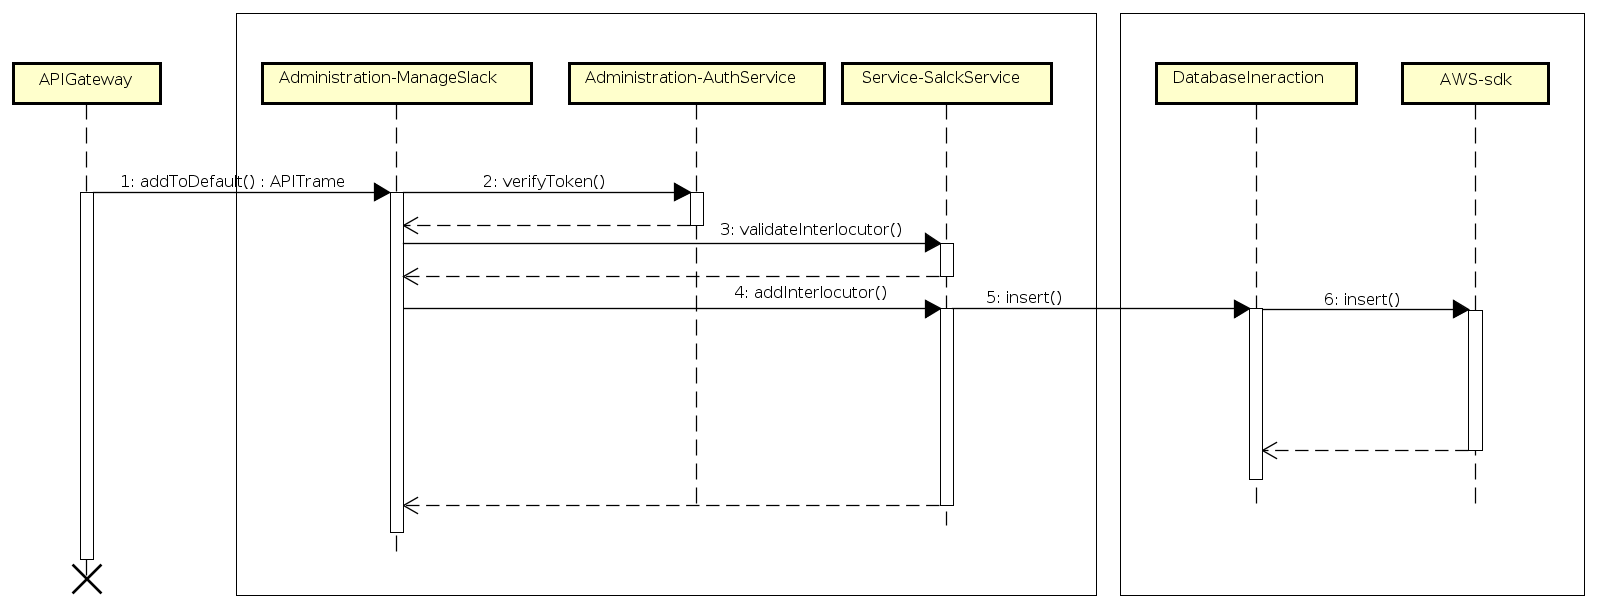
\includegraphics[width=\textwidth]{DiagrammiSequenza/Back-End/manageSlack/addtoDefault.png}
			\caption{Diagramma di sequenza - \texttt{Back-End :: Administration :: ManageSlack :: addtoDefault }}
		\end{figure}
		\begin{description}
			\item [Descrizione] Il diagramma di sequenza sopra riportato illustra la chiamata al servizio addtoDefault dell'APIGateway, che permette di aggiungere un interlocutore alla lista degli interlocutori di default.
			\item [Permessi] Amministratore autenticato.
		\end{description}

		\subsubsection{\texttt{Back-End :: Administration :: ManageSlack :: getDefualtInterlocutors}}
		\begin{figure}[!h]
			\centering
			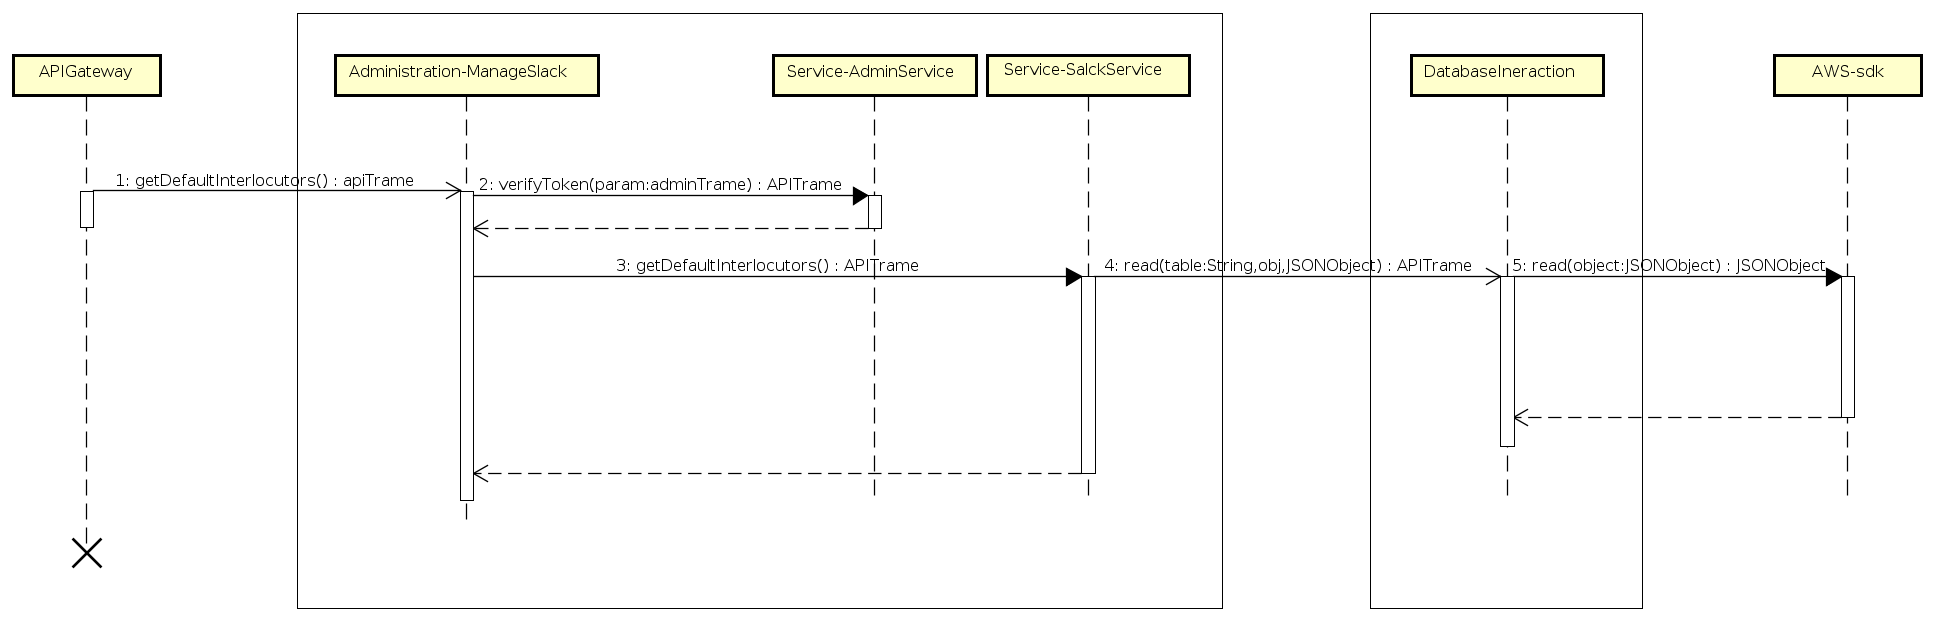
\includegraphics[width=\textwidth]{DiagrammiSequenza/Back-End/manageSlack/getDefualtInterlocutors.png}
			\caption{Diagramma di sequenza - \texttt{Back-End :: Administration :: ManageSlack :: getDefualtInterlocutors}}
		\end{figure}
		\begin{description}
			\item [Descrizione] Il diagramma di sequenza sopra riportato illustra la chiamata al servizio getDefualtInterlocutors dell'APIGateway, che restituisce la lista degli interlocutori di default assegnati.
			\item [Permessi] Amministratore autenticato.
		\end{description}

		\newpage
		\subsubsection{\texttt{Back-End :: Administration :: ManageSlack :: getInterlocutors}}
		\begin{figure}[!h]
			\centering
			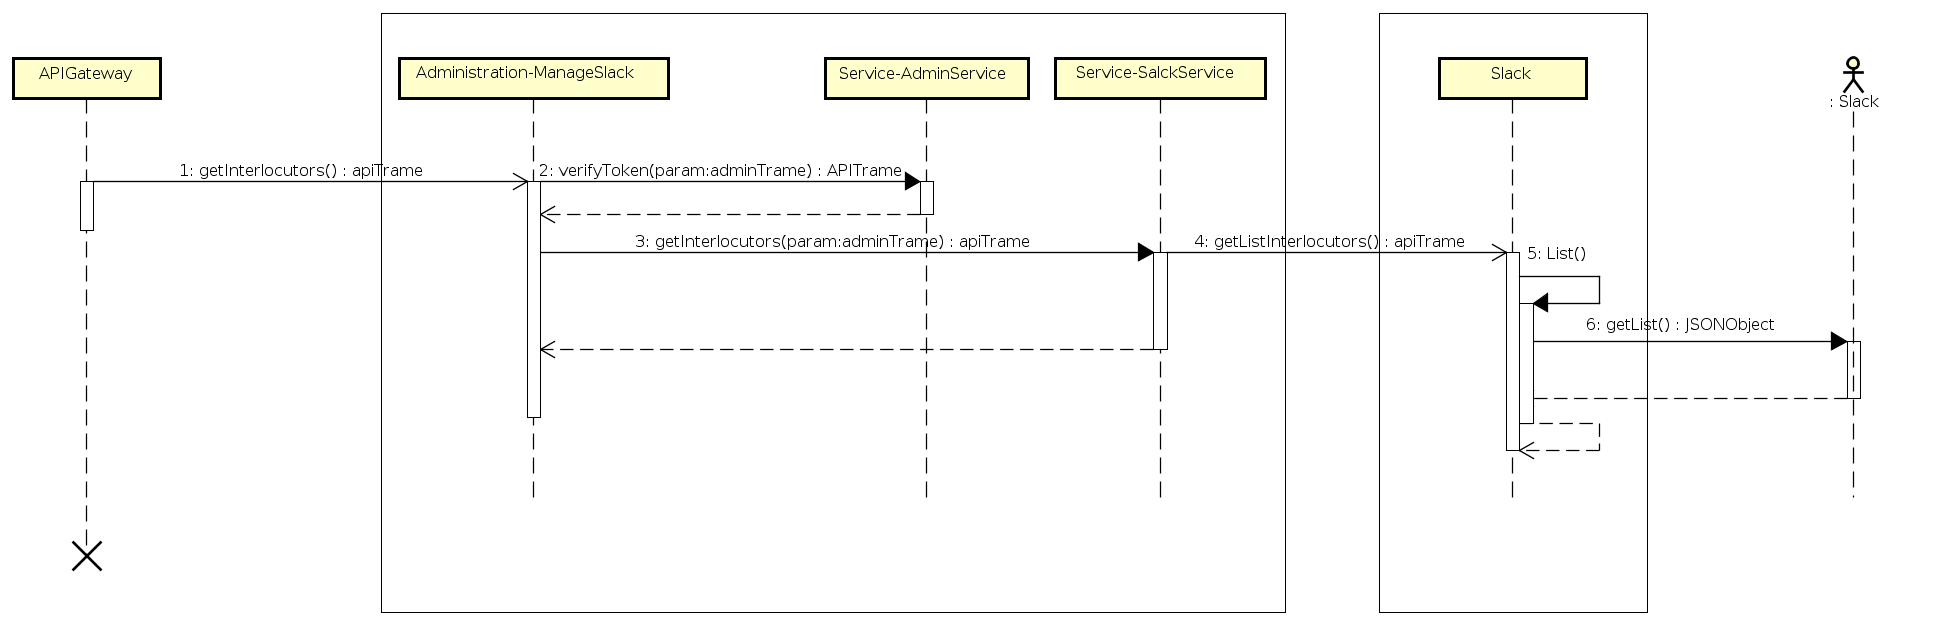
\includegraphics[width=\textwidth]{DiagrammiSequenza/Back-End/manageSlack/getInterlocutors.png}
			\caption{Diagramma di sequenza - \texttt{Back-End :: Administration :: ManageSlack :: getInterlocutors}}
		\end{figure}
		\begin{description}
			\item [Descrizione] Il diagramma di sequenza sopra riportato illustra la chiamata al servizio getInterlocutors dell'APIGateway, che restituisce la lista degli interlocutori disponibili.
			\item [Permessi] Amministratore autenticato.
		\end{description}

		\subsubsection{\texttt{Back-End :: Administration :: ManageSlack :: removeToDefault}}
		\begin{figure}[!h]
			\centering
			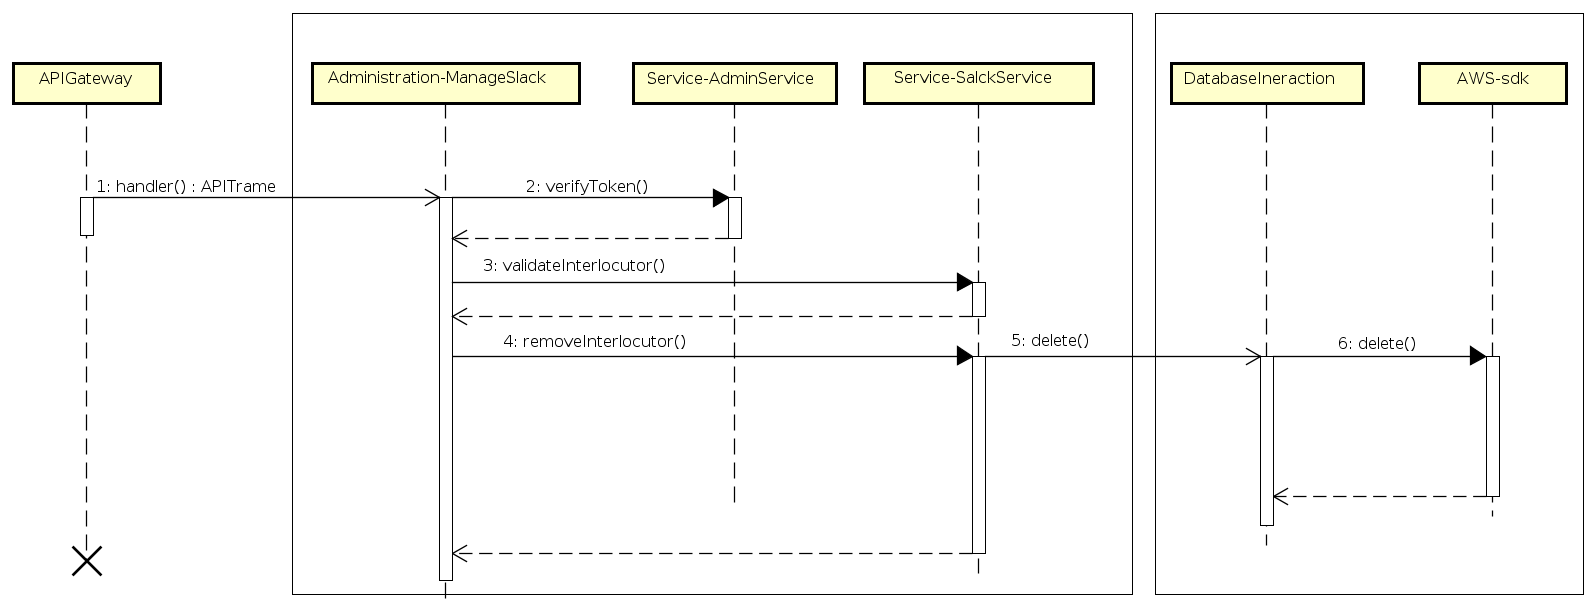
\includegraphics[width=\textwidth]{DiagrammiSequenza/Back-End/manageSlack/removeToDefault.png}
			\caption{Diagramma di sequenza - \texttt{Back-End :: Administration :: ManageSlack :: removeToDefault }}
		\end{figure}
		\begin{description}
			\item [Descrizione] Il diagramma di sequenza sopra riportato illustra la chiamata al servizio removeToDefault dell'APIGateway, che rimuove un interlocutore dal gruppo di default.
			\item [Permessi] Amministratore autenticato.
		\end{description}

		\newpage
		\subsubsection{\texttt{Alto livello Skills}}
		\begin{figure}[!h]
			\centering
			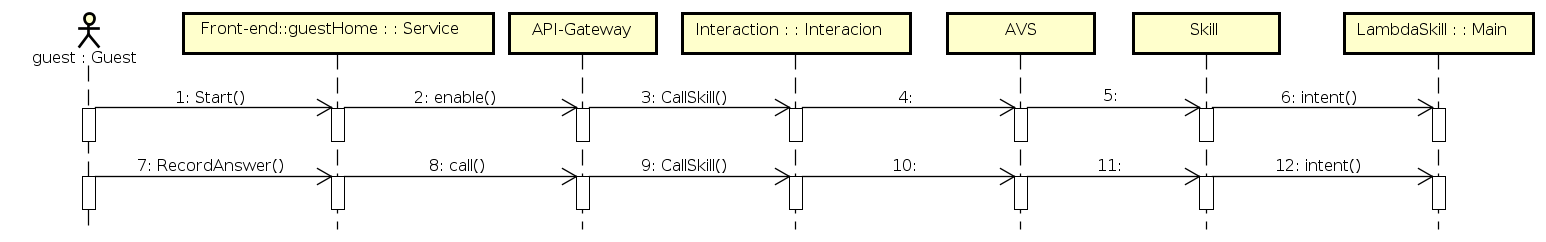
\includegraphics[width=\textwidth]{DiagrammiSequenza/Back-End/SequenzaSkills.png}
			\caption{Diagramma di sequenza - \texttt{Alto livello Skills }}
		\end{figure}
		\begin{description}
			\item [Descrizione] Il diagramma di sequenza sopra riportato illustra la catena di chiamate che vengono effettuate quando un ospite interagisce con l'AV. Viene visualizzata una chiamata di inizializzazione ed una chiamata tipo per l'interazione.
		\end{description}

\end{document}
